\newpage
\section{Results}

\subsection{MILP Multi-Year Grid Optimization and Asset Planning}

\subsubsection*{A. System Configuration}
The example grid consists of five interconnected buses, each hosting a mix of generation, load, 
and storage assets (see Table~\ref{tab:config-storages}). The asset portfolio includes 
dispatchable thermal generators (with varying capital costs and mutual exclusivity constraints), 
renewables (solar and wind), and an array of storage systems. 

Unlike traditional static approaches, all assets are available as a *candidate pool* ; the MILP 
optimization selects which assets to deploy, and when, based on system needs and economics. 
Multiple candidate assets may be located at the same bus, reflecting both technical redundancy 
and the physical or geographic constraints of real networks. The line capacities and susceptances 
are configured to ensure a realistic representation of typical mid-scale regional grids.

\begin{table}[h]
    \centering
    \begin{tabular}{p{1.5cm} p{3.5cm} p{1.5cm} p{2.5cm} p{2.5cm}}
    \textbf{ID} & \textbf{Type} & \textbf{Bus} & \textbf{Lifetime [yrs]} & \textbf{CAPEX [k\$]} \\
    \hline
    1001 & Thermal Generator 1 & 1 & 25 & 10 \\
    1002 & Thermal Generator 2 & 1 & 30 & 10 \\
    1003 & Solar Generator 1 & 1 & 25 & 6000 \\
    1004 & Solar Generator 2 & 2 & 25 & 8000 \\
    1005 & Wind Generator 2 & 4 & 25 & 7000 \\
    1006 & Solar Generator 3 & 3 & 25 & 4000 \\
    1007 & Solar Generator 1 & 4 & 25 & 8000 \\
    1008 & Wind Generator 3 & 4 & 25 & 8000 \\
    1009 & Wind Generator 4 & 4 & 25 & 8500 \\
    1010 & Thermal Alt. 1 & 1 & 4 & 70 \\
    1020 & Thermal Alt. 2 & 1 & 25 & 950 \\
    \end{tabular}
\end{table}

\begin{table}[h]
    \centering
    \begin{tabular}{p{1.5cm} p{3.5cm} p{1.5cm} p{2.5cm} p{2.5cm}}
    \textbf{ID} & \textbf{Type} & \textbf{Bus} & \textbf{Lifetime [yrs]} & \textbf{CAPEX [k\$]} \\
    \hline
    3001 & Storage 1 & 2 & 10 & 3.5 \\
    3002 & Storage 2 & 3 & 12 & 7.85 \\
    3003 & Storage 3 & 1 & 11 & 4.25 \\
    3004 & Storage 4 & 4 & 10 & 4.65 \\
    \end{tabular}
    \caption{Summary of Available Storage and Generations Assets in Grid Model}
    \label{tab:config-storages}
\end{table}

To ensure the system remains responsive to evolving needs, demand is modeled to grow 
at a compound rate of 3\% annually for the first 15 years, increasing to 5\% per year 
thereafter. This results in a tripling of total load by year 30, imposing continuous 
pressure to replace 'about-to-die' assets in a timely manner.

\begin{figure}[h!]
    \centering
    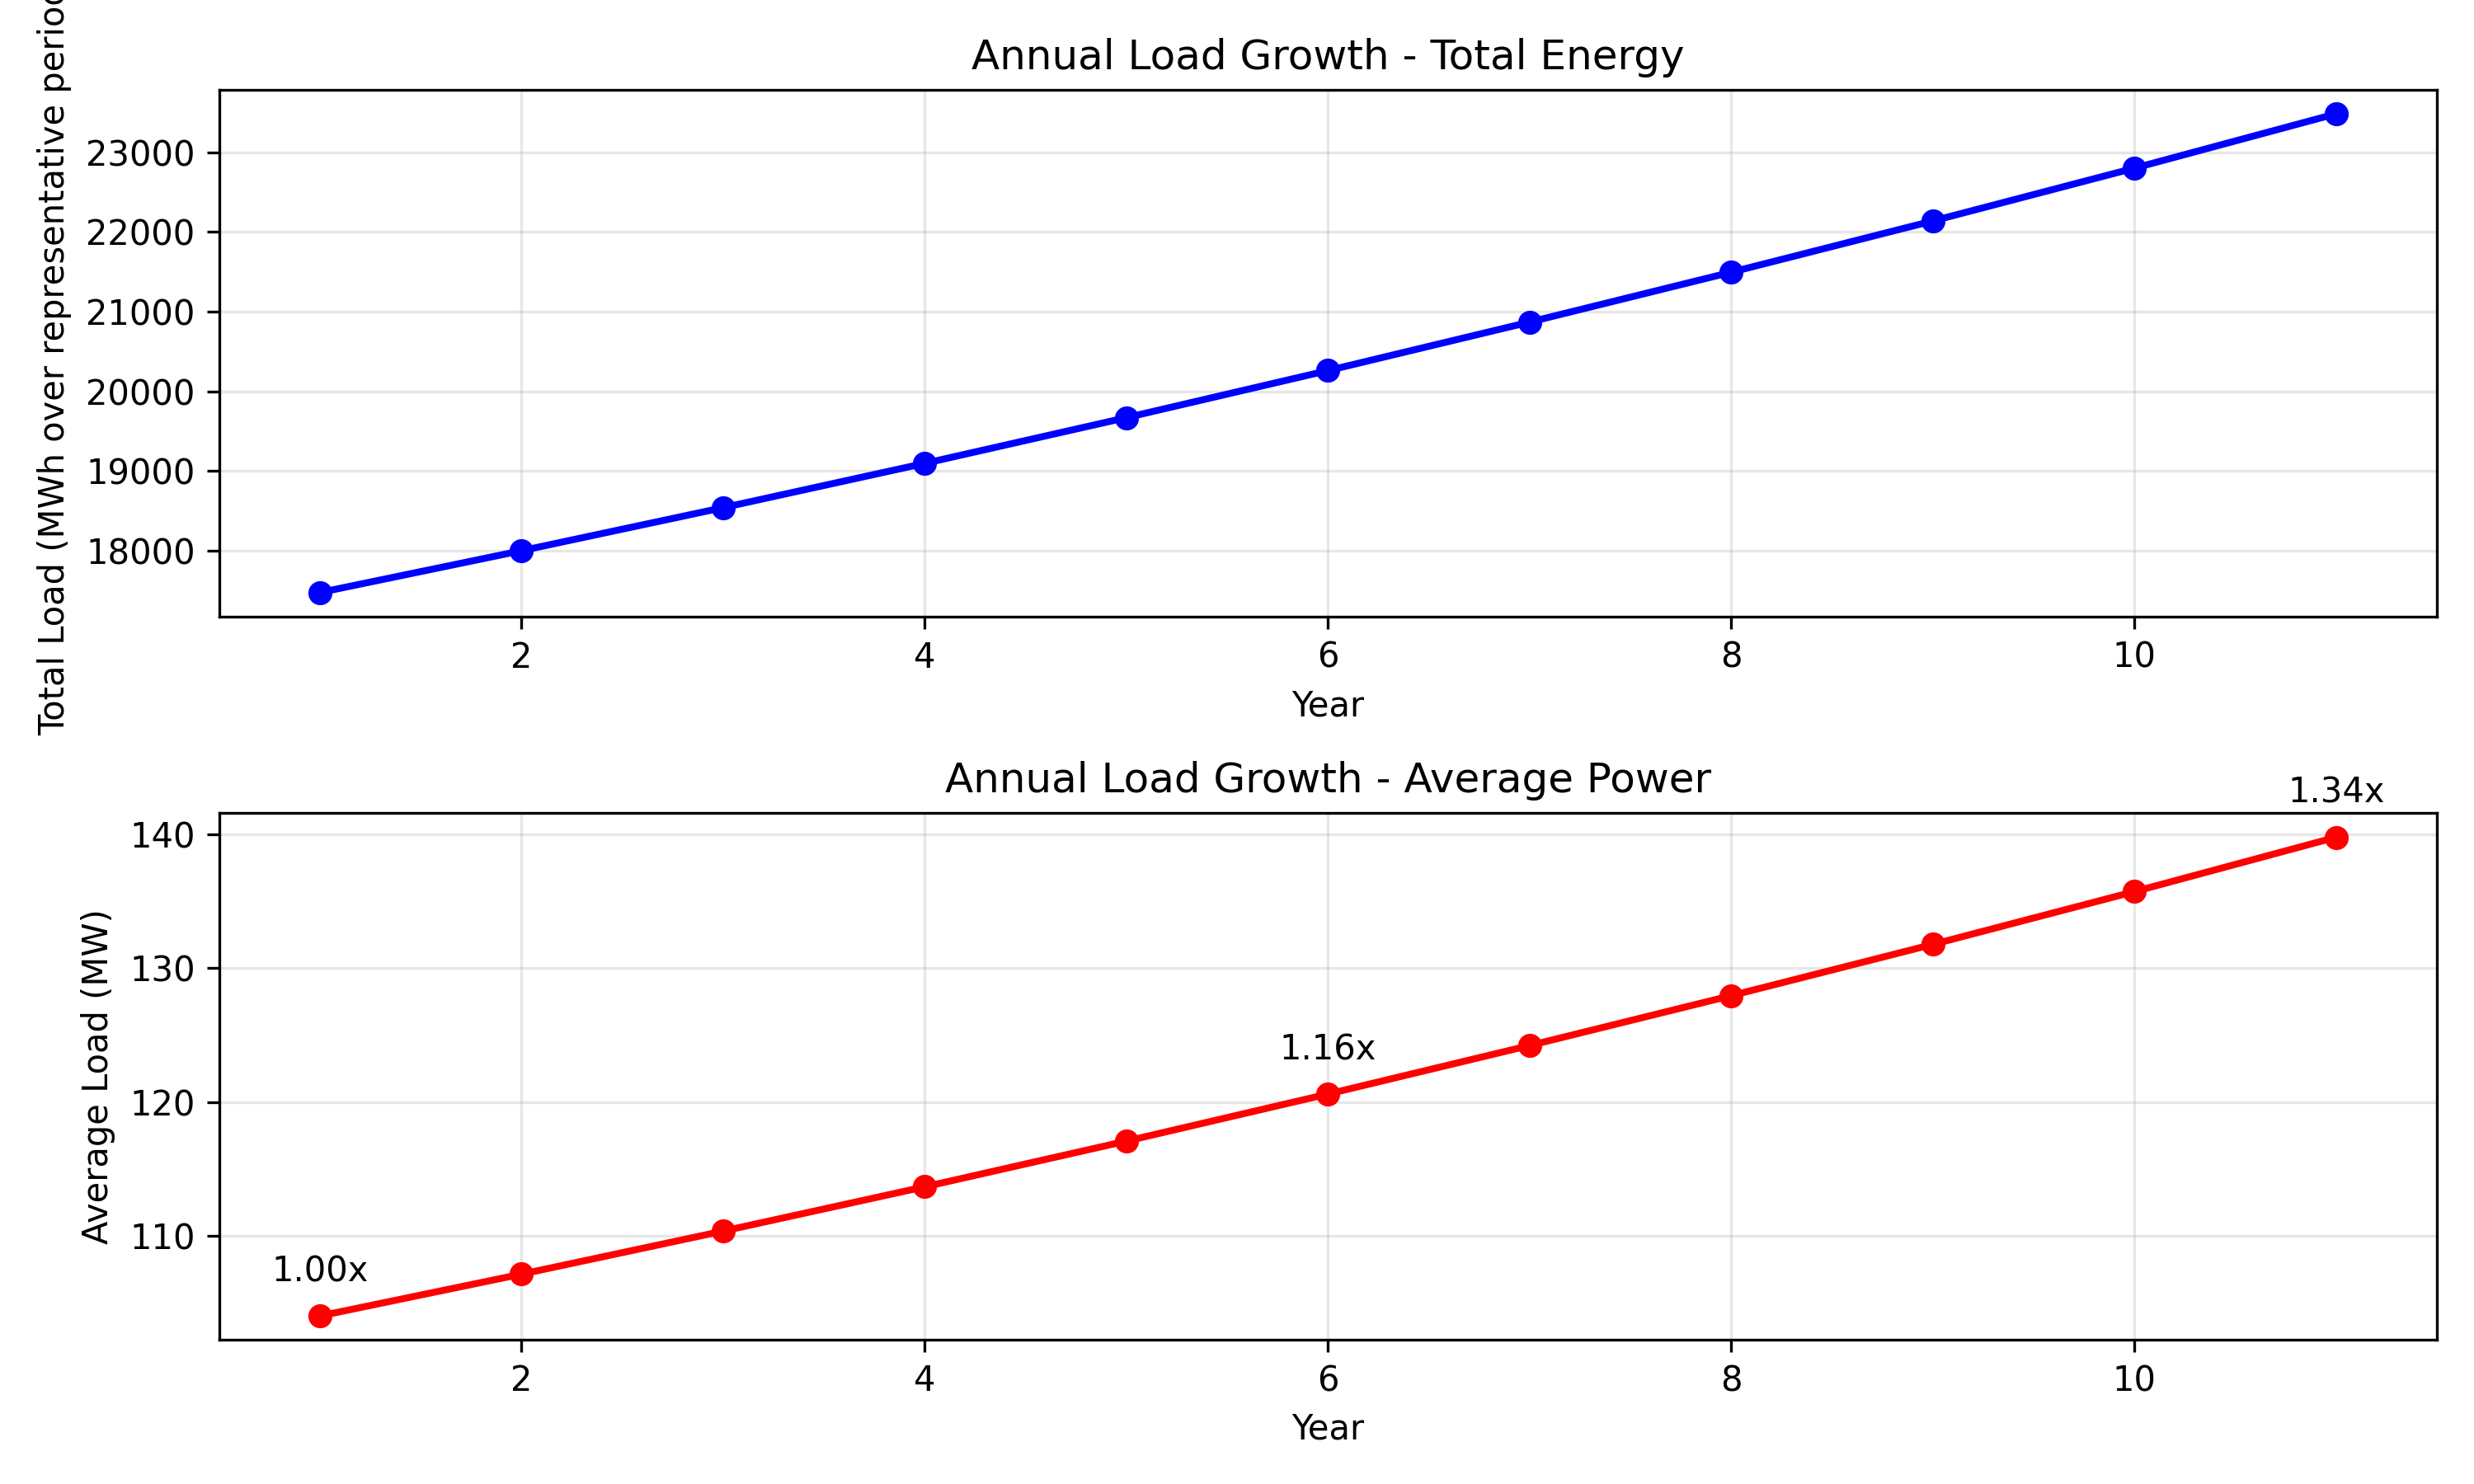
\includegraphics[width=0.8\textwidth]{images/annual_load_growth.png}
    \caption{Annual load growth over the 30-year horizon.}
    \label{fig:annual_load_growth}
\end{figure}

\subsubsection*{B. Planning Horizon}
The adoption of a mixed-integer linear programming (MILP) approach for multi-year planning enables 
the model to co-optimize both investment and operational decisions across the entire horizon. 
Unlike previous LP-based, scenario-driven studies, the MILP directly answers \textit{when} and 
\textit{where} to install, replace, or retire each candidate asset to meet both optimal economic and 
load fulfillment objectives.

\begin{figure}[h!]
    \centering
    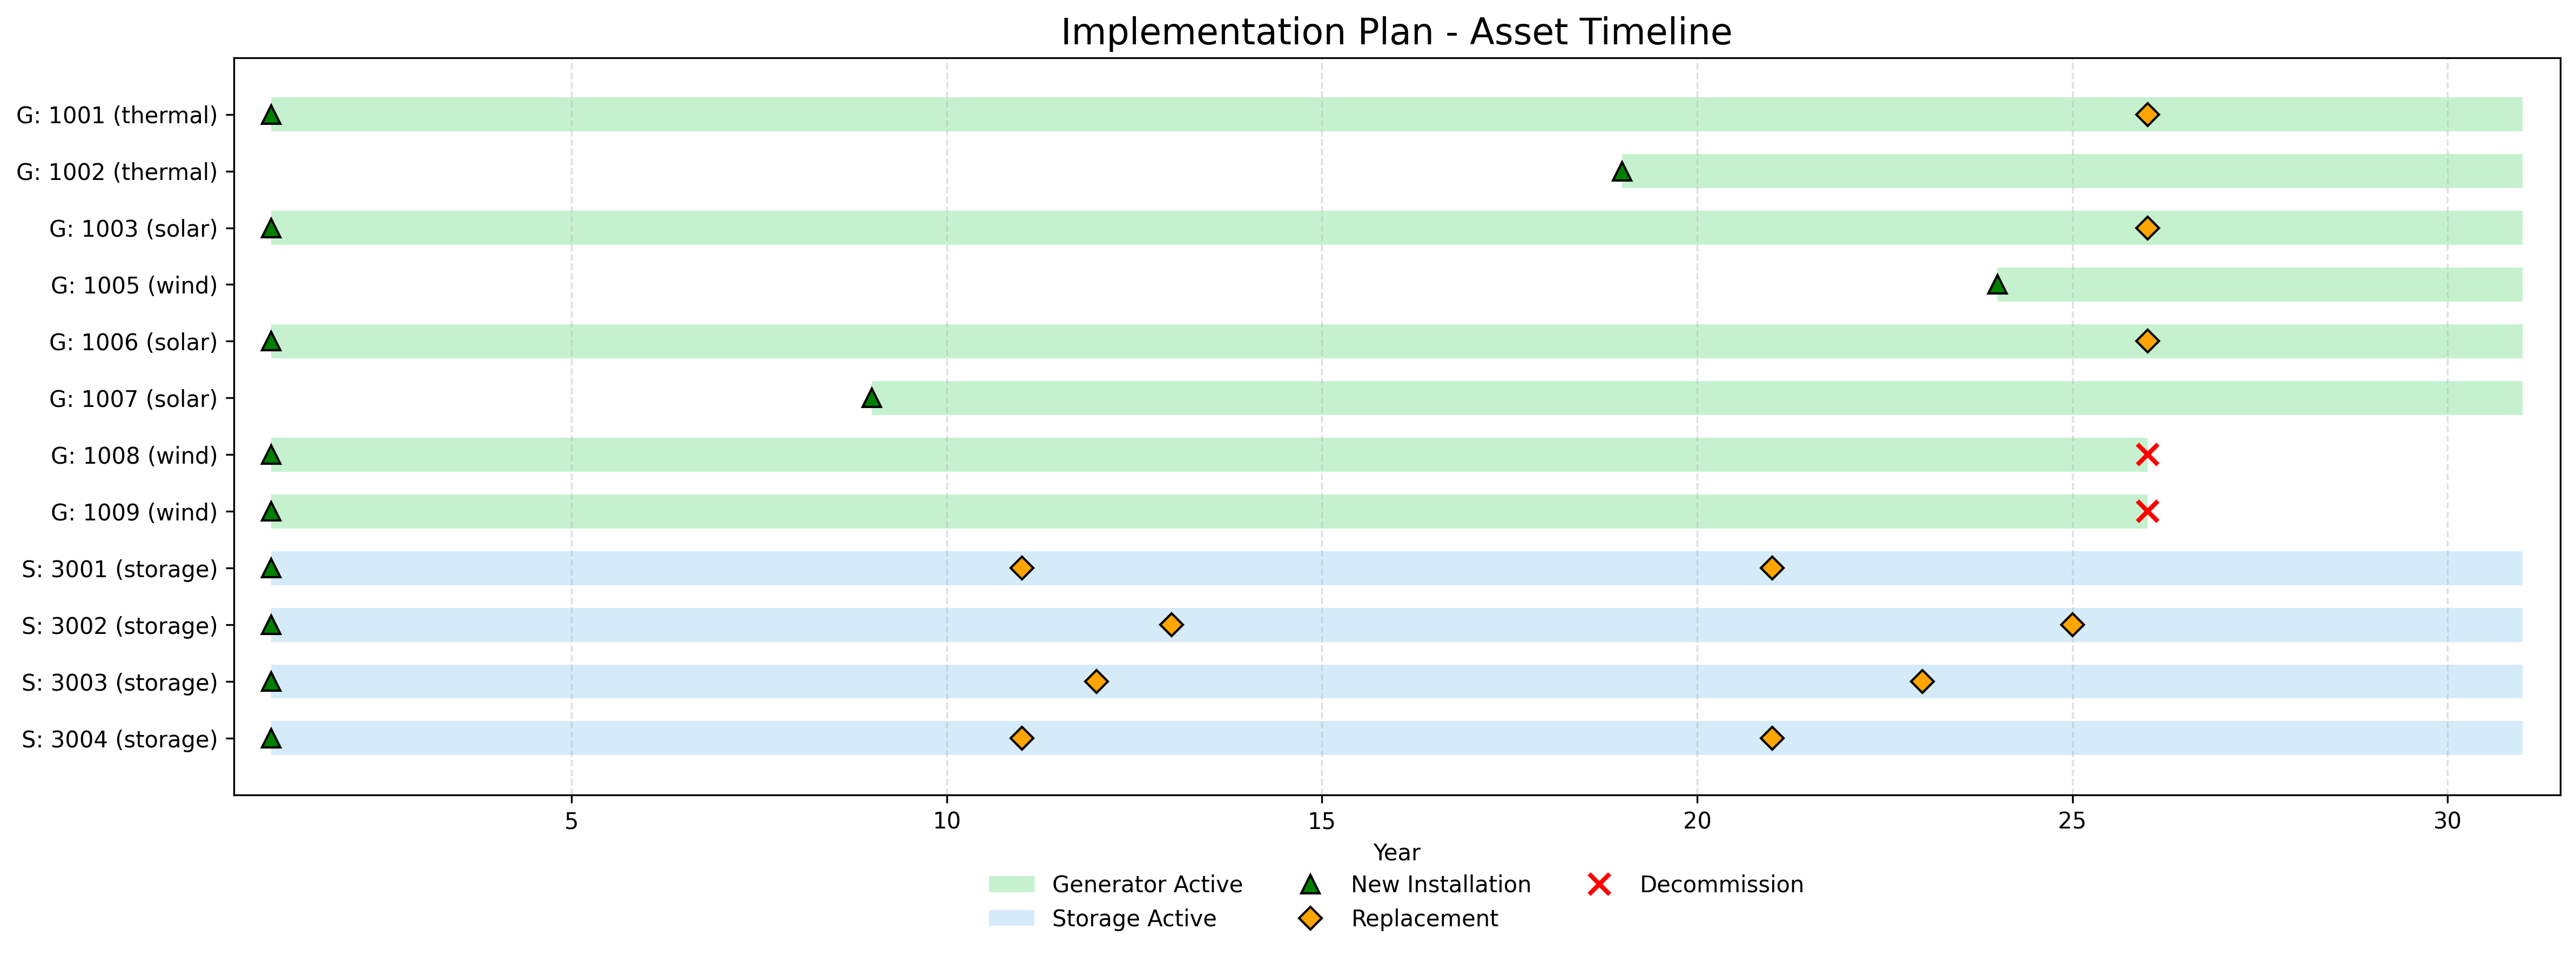
\includegraphics[width=\textwidth]{images/asset_timeline.png}
    \caption{Asset timeline over the 30-year planning horizon}
    \label{fig:asset_timeline}
\end{figure}

Figure~\ref{fig:asset_timeline} summarizes the resulting implementation and replacement schedule 
for all key assets. We notice that all available storage assets are commissioned in the first period, 
while new renewables and thermal units are deployed as demand and system needs dictate. The 
optimization naturally schedules asset replacements at the end of their technical lifetimes, 
reflecting not only load growth but also asset aging.

\textit{Analysis:}
\vspace{-0.4em}
\begin{itemize}
    \item The optimization seems to prefer early deployment of 'green' assets such as solar, wind, 
    and storage despite their relatively shorter lifetimes. It is proof of the economic relevance.
    \item Large-scale thermal investments are deferred until later in the planning horizon 
    (e.g., year 19 for Thermal Generator 2). This is likely due to the fact that thermal assets 
    are more expensive to build and operate.
    \item Storages also showcase their economic relevance beside their known convinience. All available storages
    are installed in the first period already.
    \item The model seems to be able to handle the load growth and the asset aging. It is able to 
    replace the assets at the end of their technical lifetimes and increase the number of assets.
\end{itemize}

\subsubsection*{C. Energetic Mix}
The new MILP model enables a detailed examination of how the system's energetic mix evolves 
over time. While seasonal analysis (summer vs. winter) was already feasible in the previous 
LP-based approach, the multi-year MILP framework now makes it possible to directly compare 
the system’s dispatch between the first and last years of the planning horizon.

% \begin{figure}[h!]
%     \centering
%     \begin{subfigure}{0.5\textwidth}
%         \centering
%         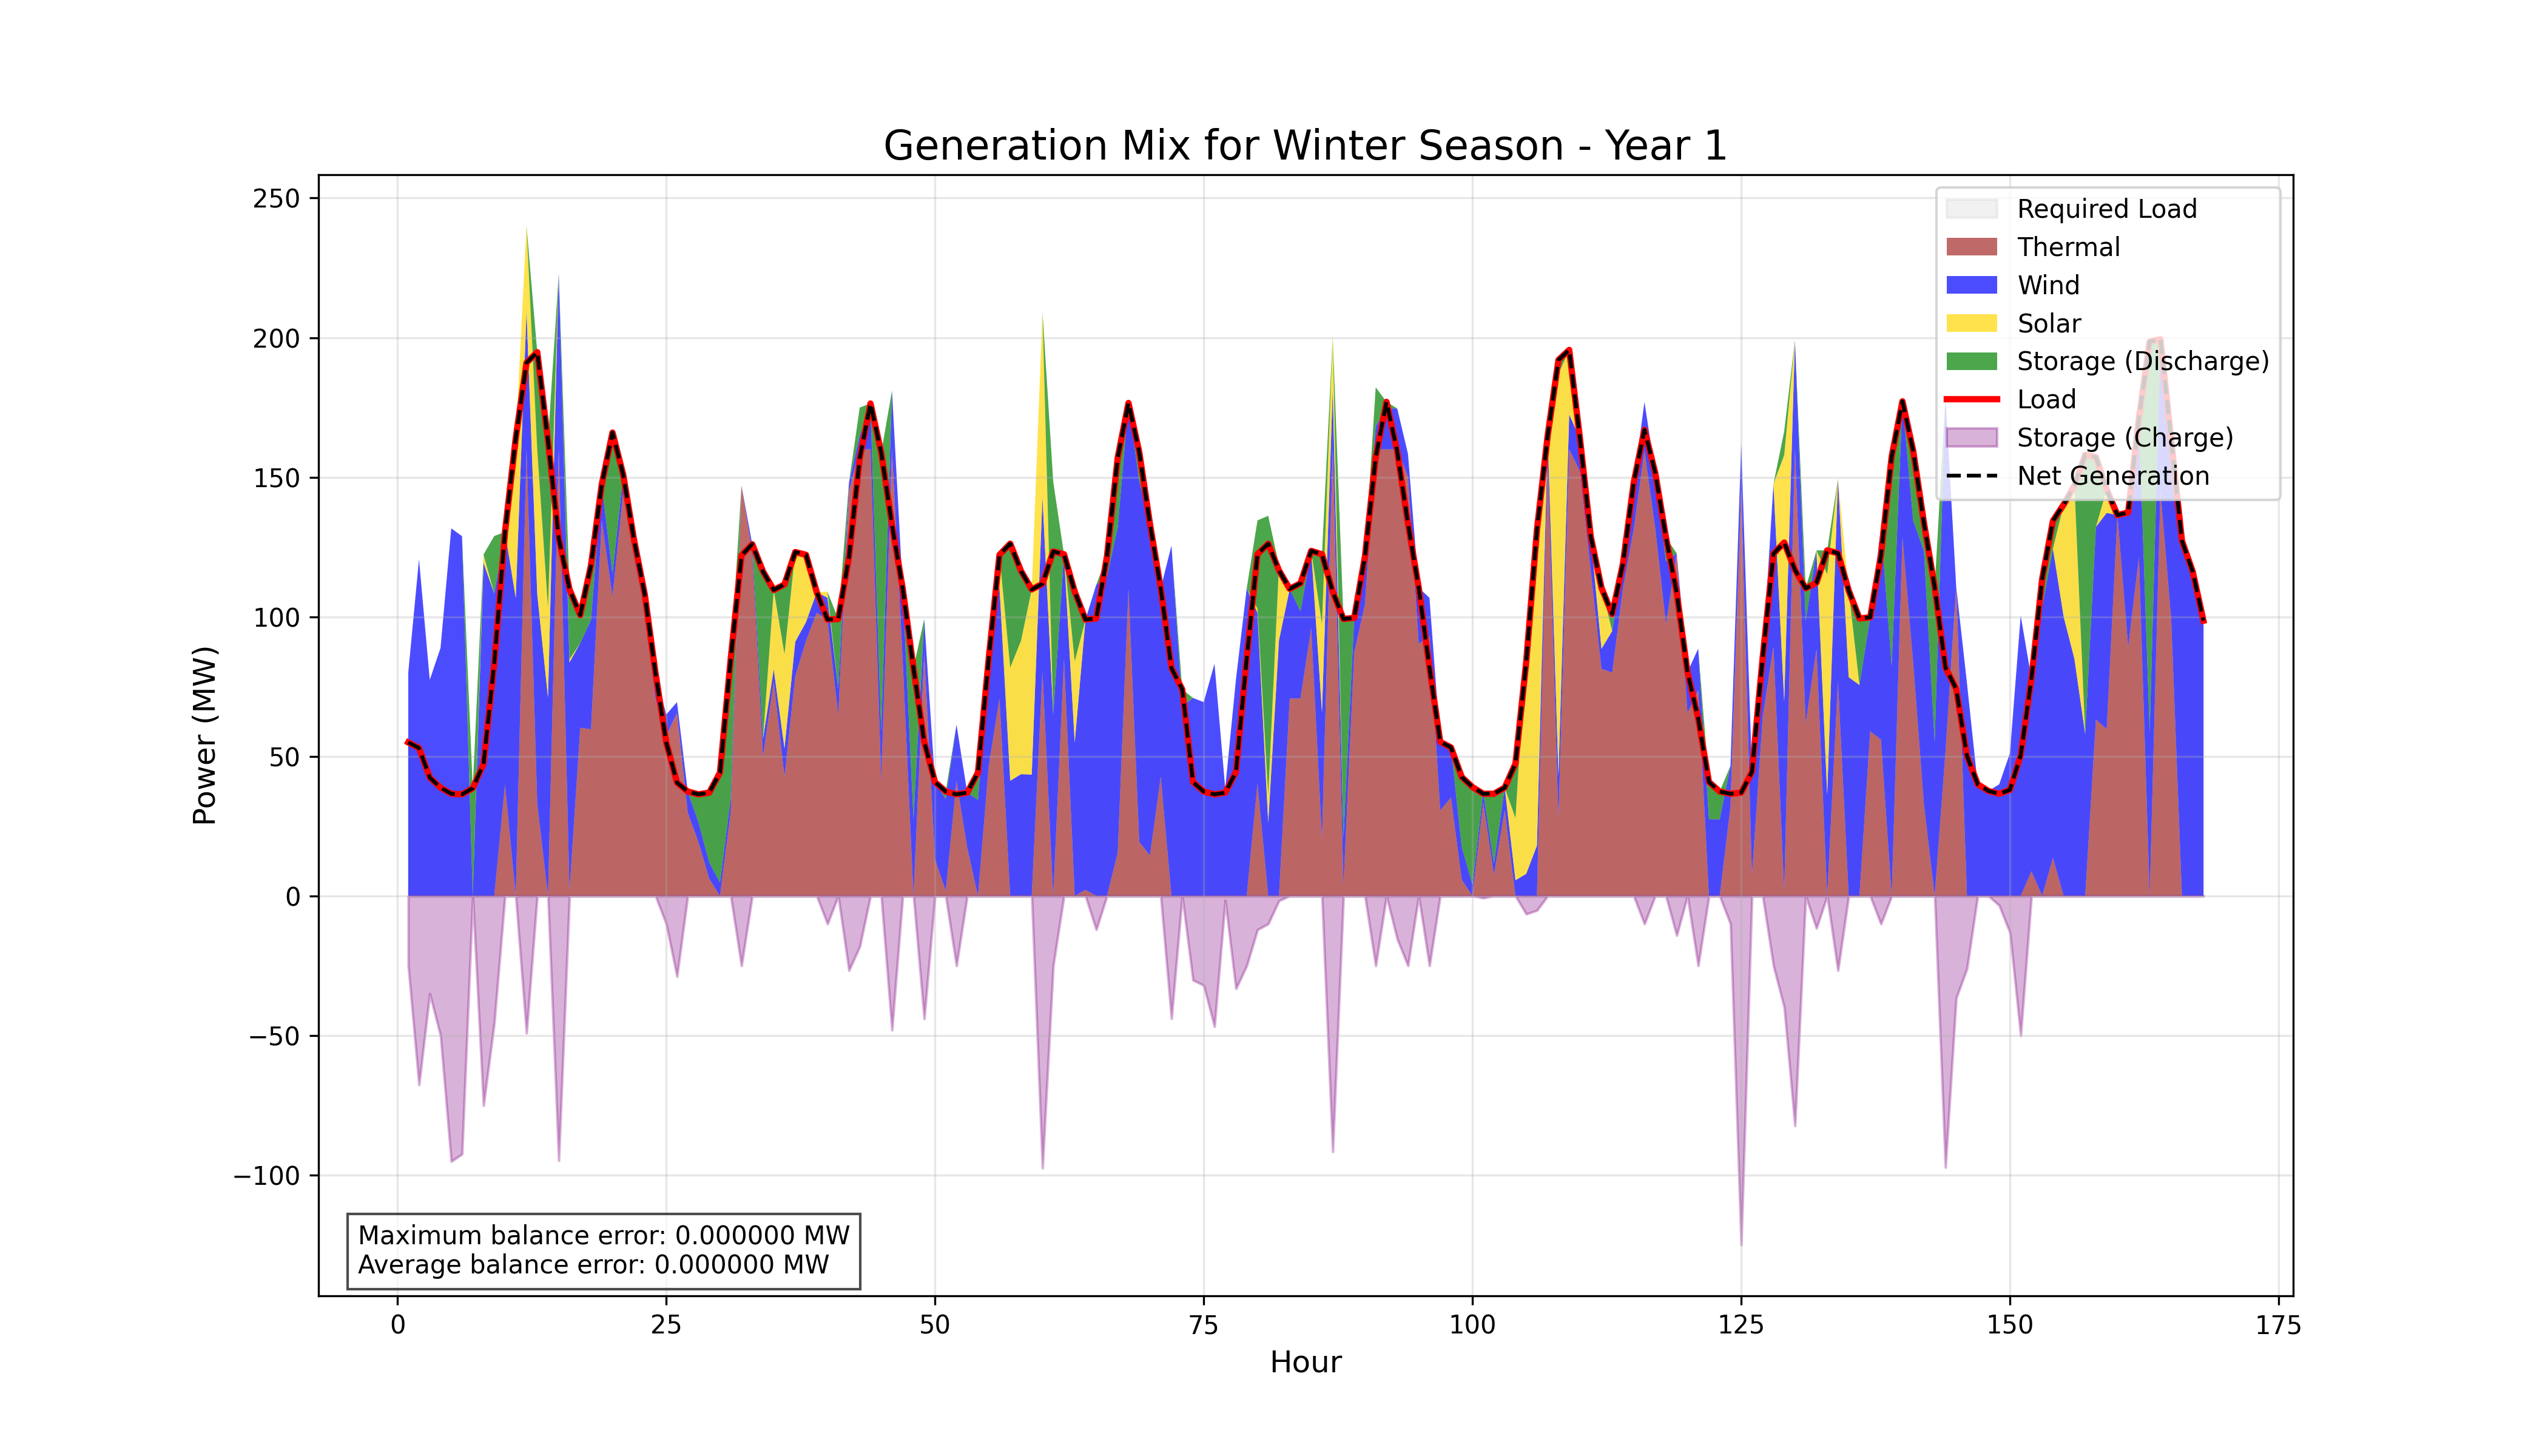
\includegraphics[width=\textwidth]{images/winter_mix_year1.png}
%         \caption{Winter, Year 1}
%         \label{fig:winter_mix_year1_sub}
%     \end{subfigure}
%     \hfill
%     \begin{subfigure}{0.5\textwidth}
%         \centering
%         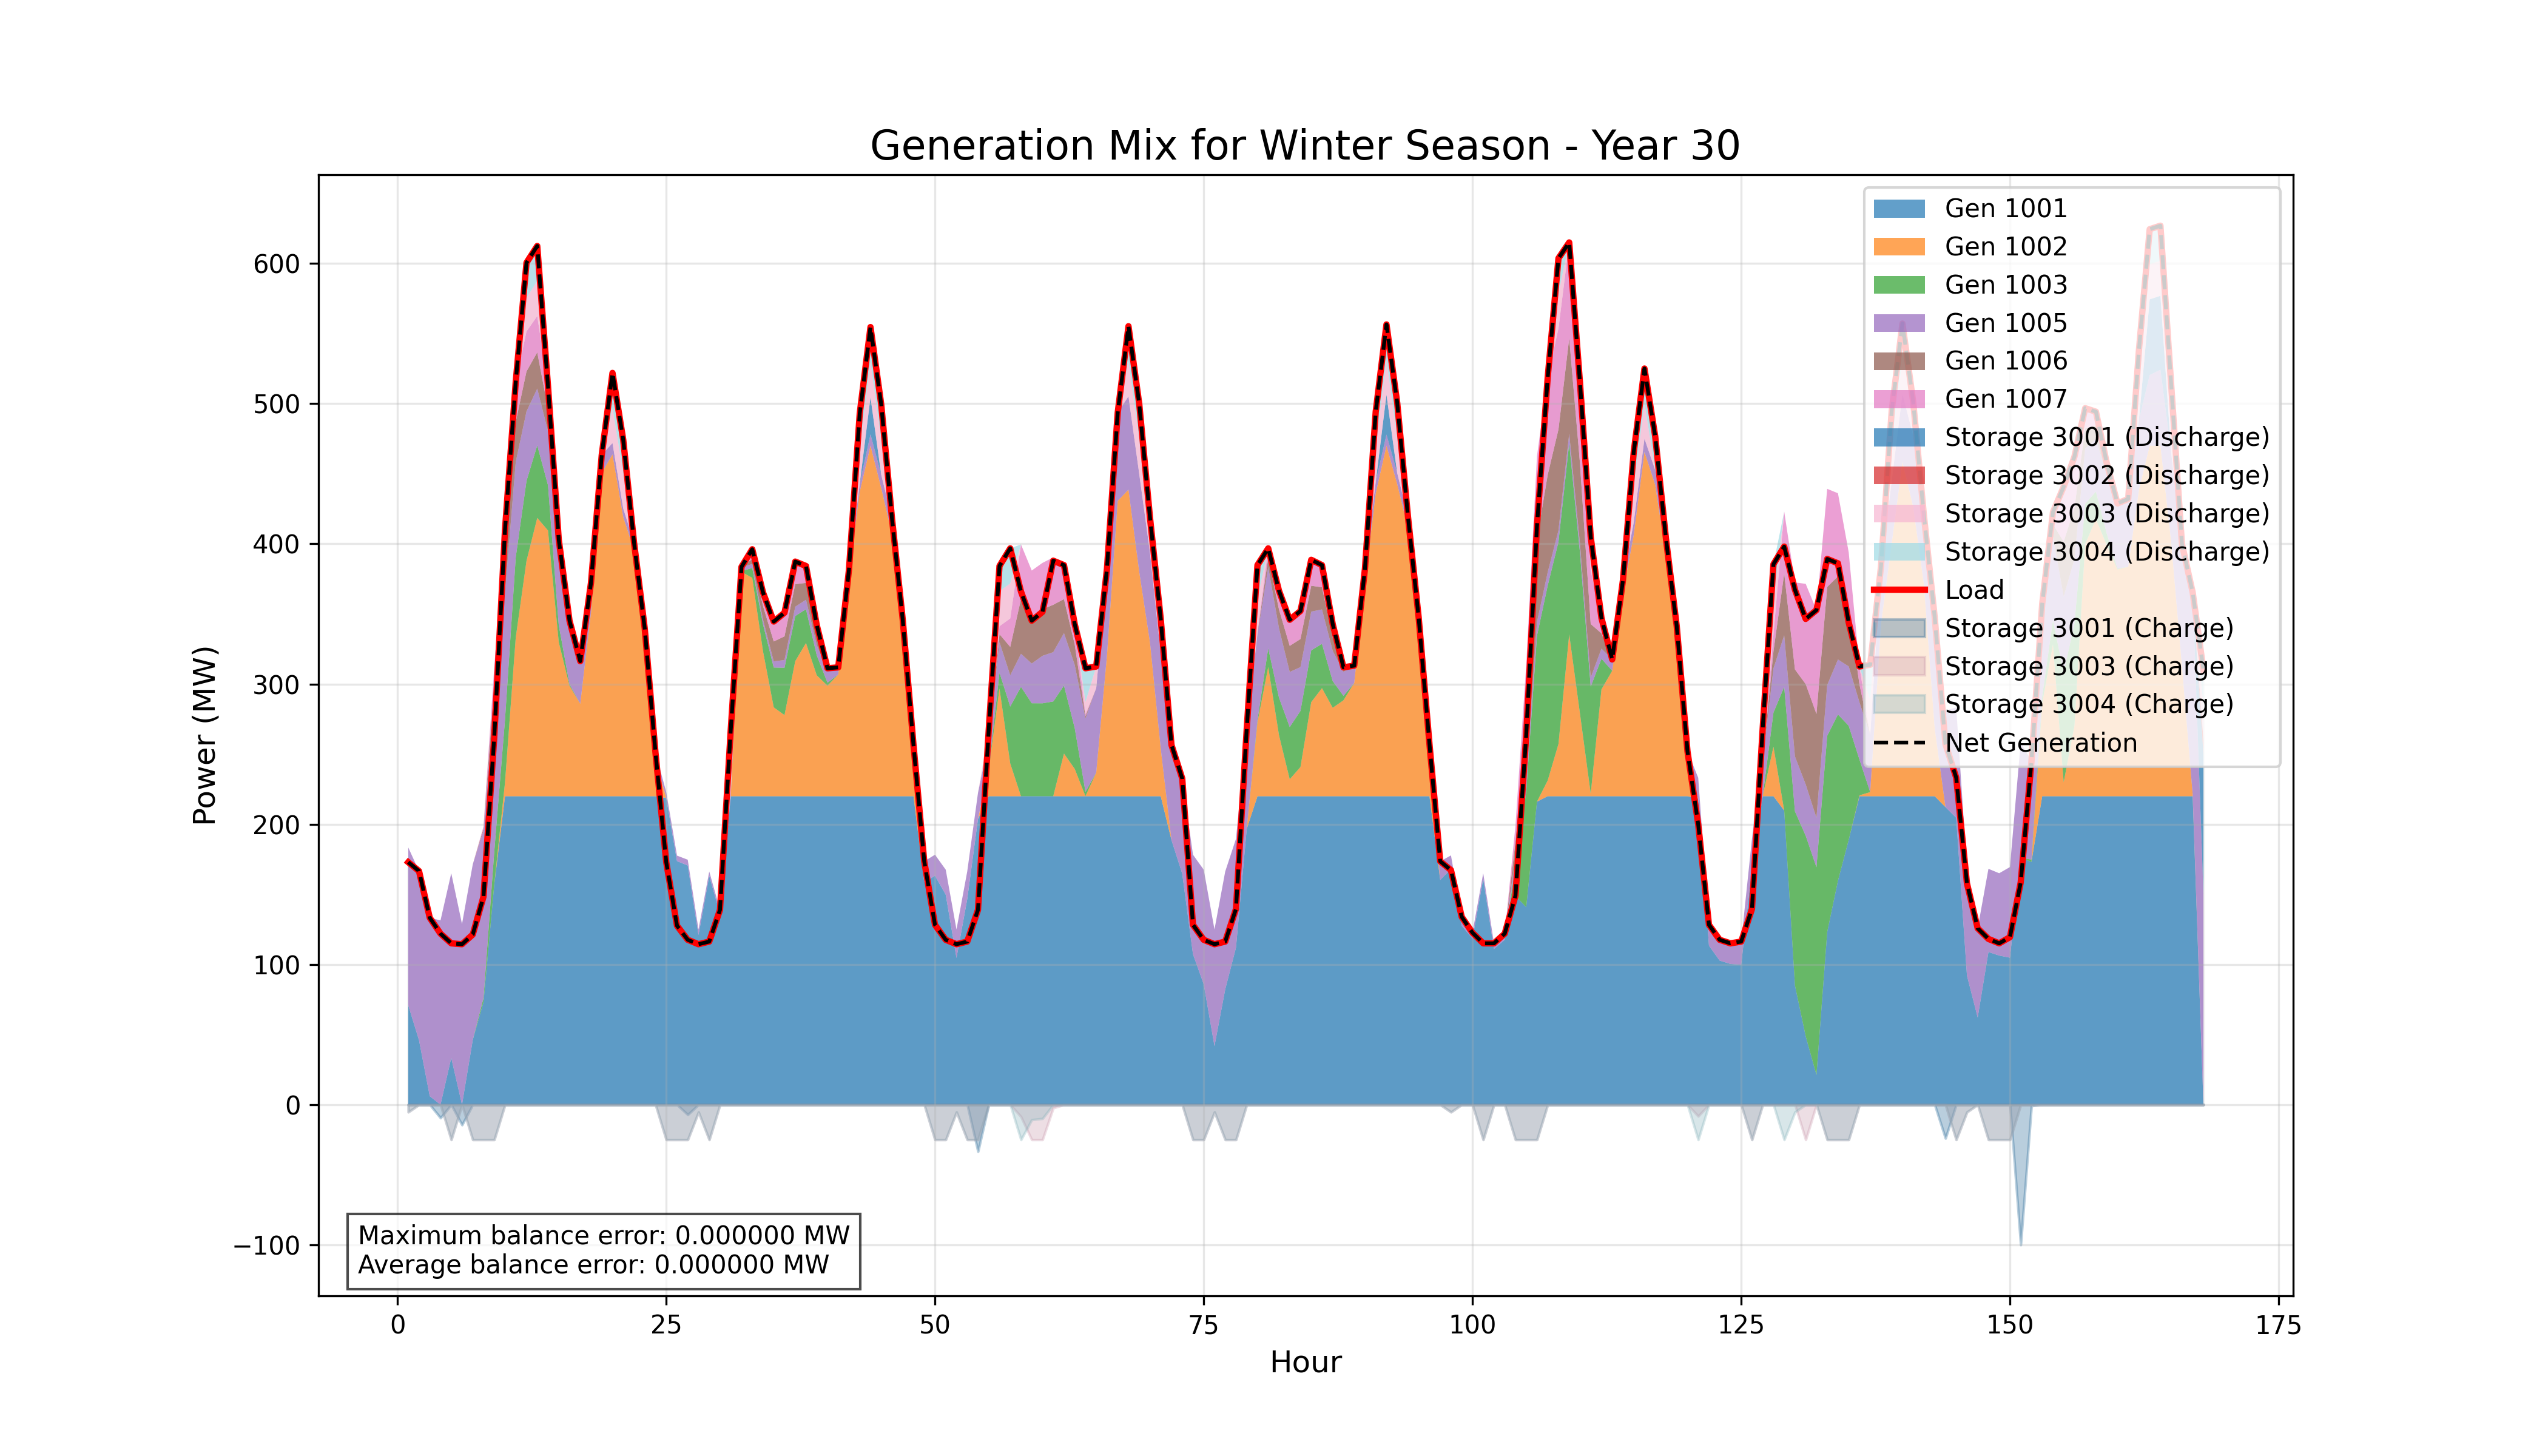
\includegraphics[width=\textwidth]{images/winter_mix_year30.png}
%         \caption{Winter, Year 30}
%         \label{fig:winter_mix_year30_sub}
%     \end{subfigure}
%     \vskip\baselineskip
%     \begin{subfigure}{0.5\textwidth}
%         \centering
%         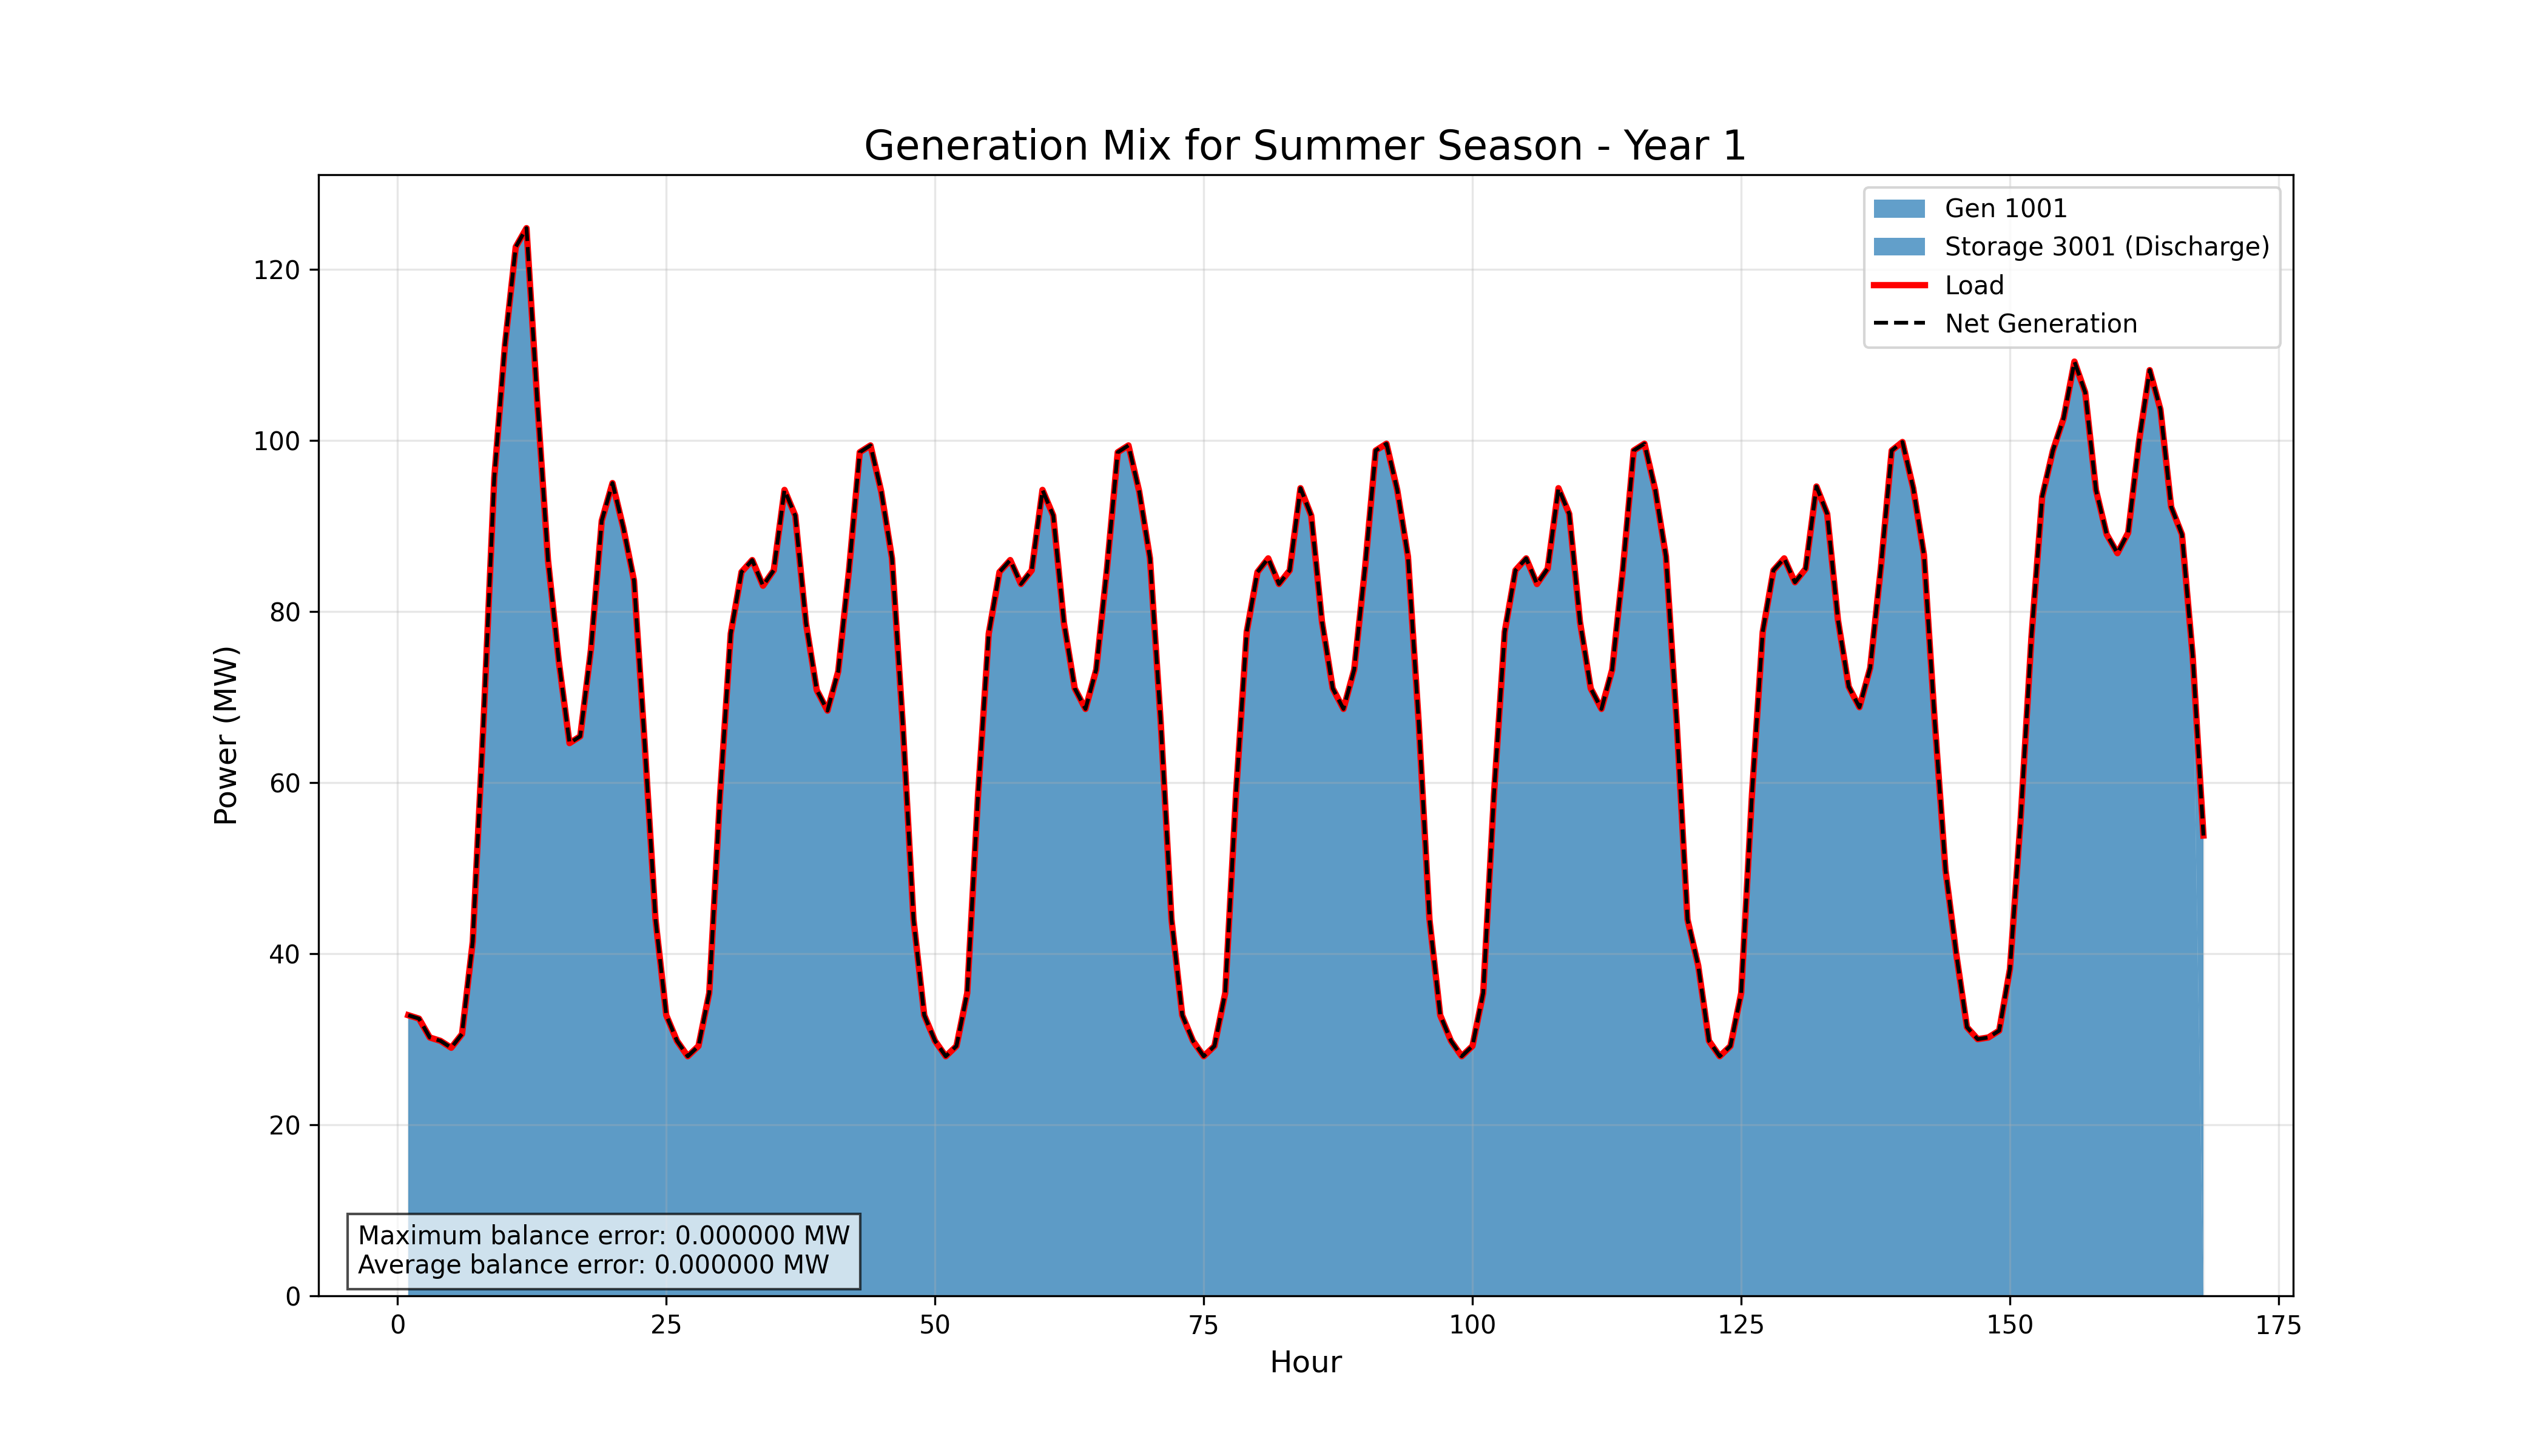
\includegraphics[width=\textwidth]{images/summer_mix_year1.png}
%         \caption{Summer, Year 1}
%         \label{fig:summer_mix_year1_sub}
%     \end{subfigure}
%     \hfill
%     \begin{subfigure}{0.5\textwidth}
%         \centering
%         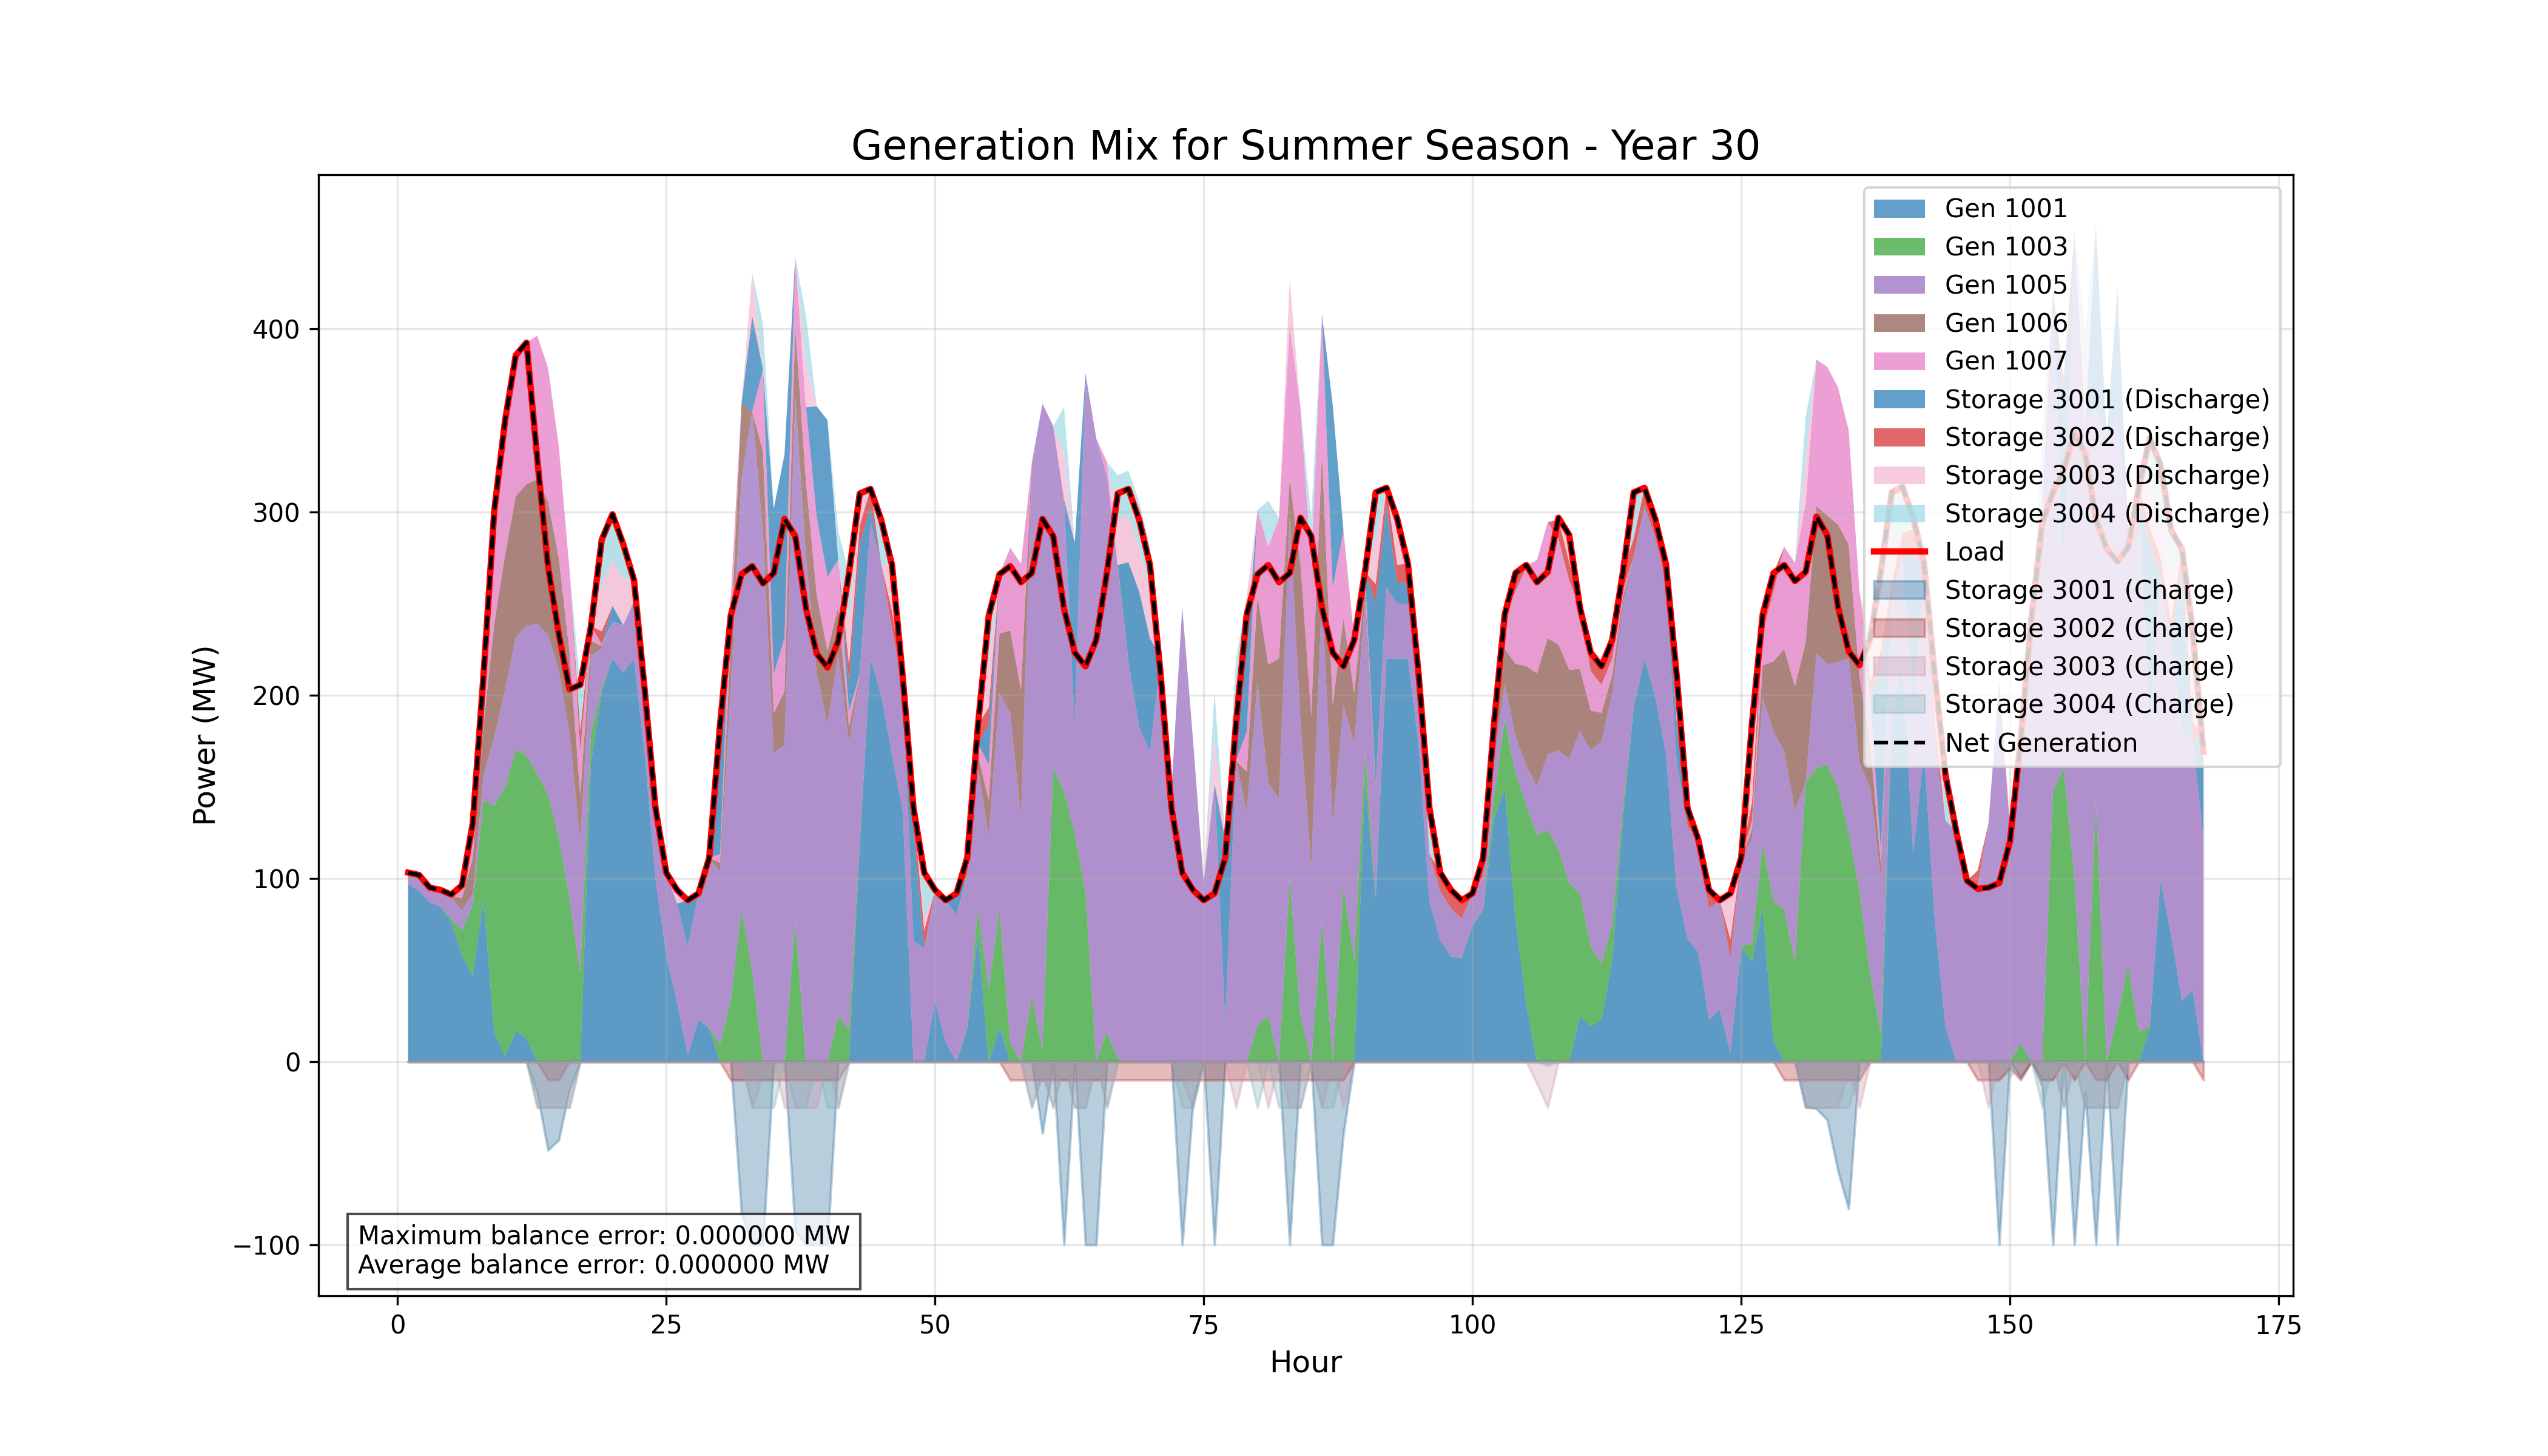
\includegraphics[width=\textwidth]{images/summer_mix_year30.png}
%         \caption{Summer, Year 30}
%         \label{fig:summer_mix_year30_sub}
%     \end{subfigure}
%     \caption{Comparison of generation mix during representative weeks in Year 1 and Year 30 for both winter and summer.}
%     \label{fig:seasonal_mix_comparison}
% \end{figure}

Figures~\ref{fig:winter_mix_year1} and~\ref{fig:winter_mix_year30} illustrate the 
generation mix during a representative winter week in Year 1 and Year 30, respectively. 
Analogous plots for a summer week are shown in Figures~\ref{fig:summer_mix_year1} 
and~\ref{fig:summer_mix_year30}. We notice a significant difference in the asset utilization 
and the adaptability of the dispatch strategy across variable demands driven here by either 
the season or the load growth. Plot's Y-scales (Power [MW]) are not identical accross results.

\newpage
\begin{figure}[h!]
    \centering
        \centering
        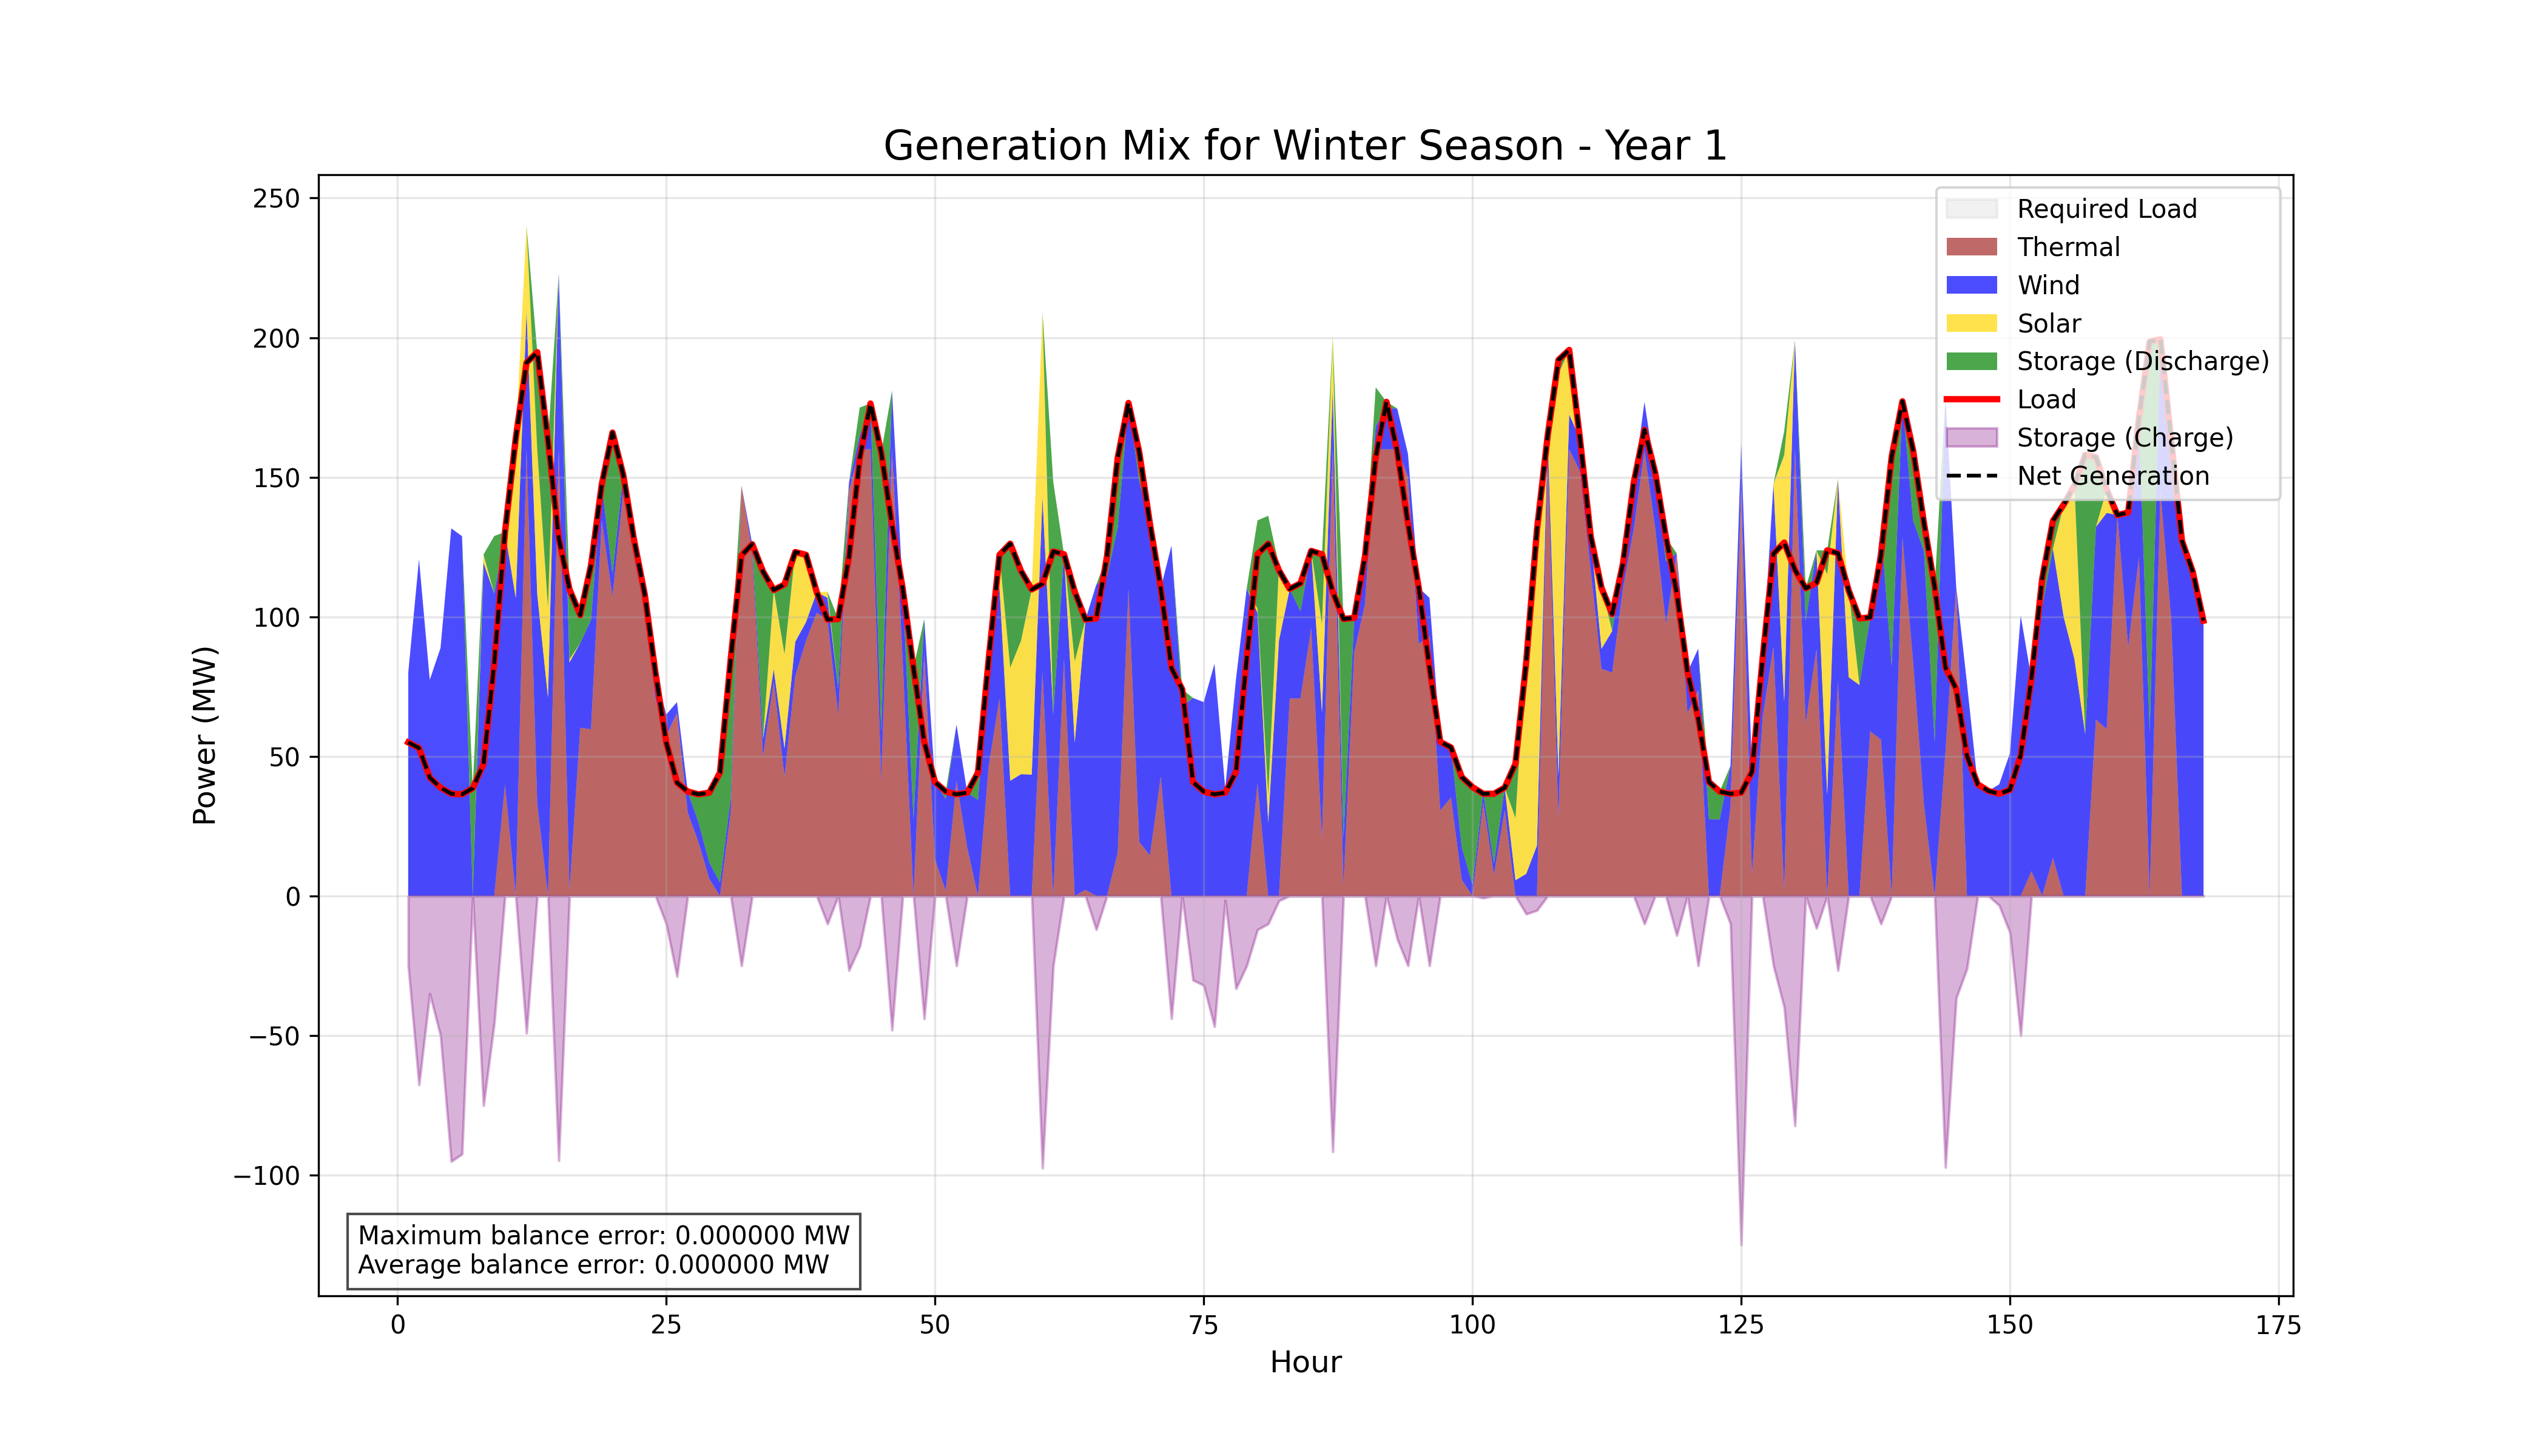
\includegraphics[width=0.85\textwidth]{images/winter_mix_year1.png}
        \caption{Winter week, Year 1}
        \label{fig:winter_mix_year1}
\end{figure}
% Dispatch is dominated by thermal generation. 
% Renewables and storage are present but secondary, with storage mostly handling short-term balancing
\begin{figure}[h!]
    \centering
        \centering
        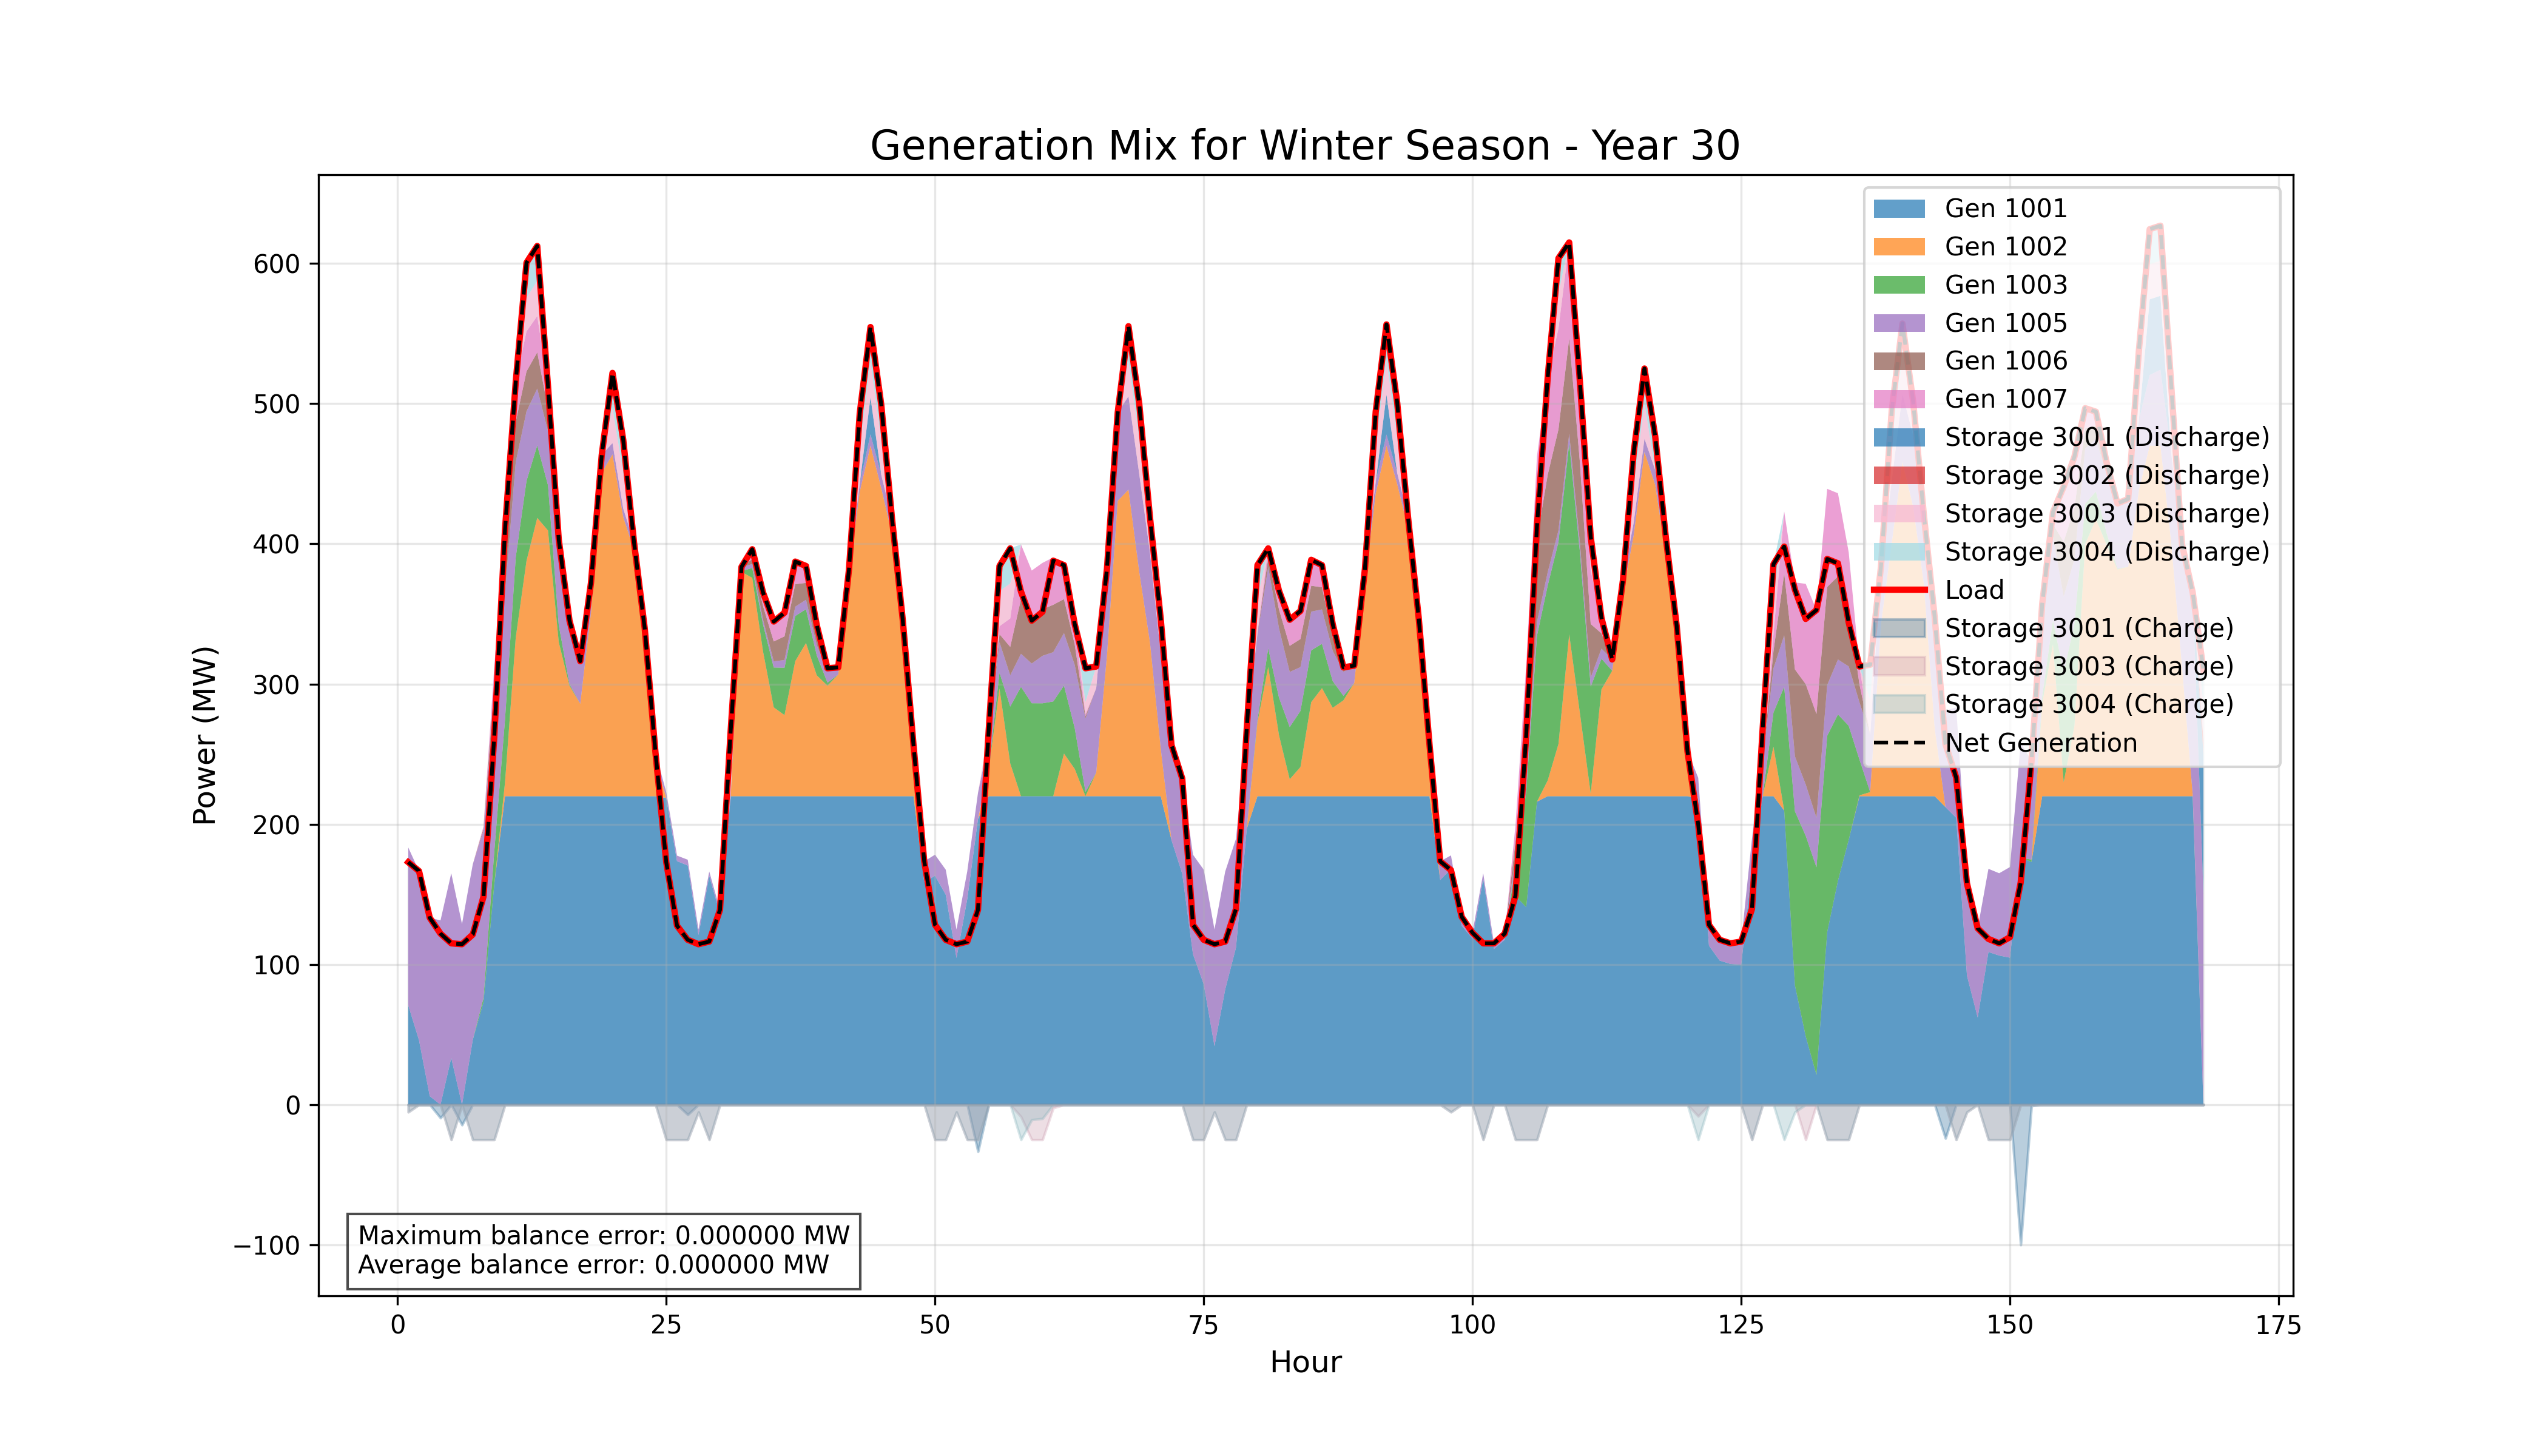
\includegraphics[width=0.85\textwidth]{images/winter_mix_year30.png}
        \caption{Winter week, Year 30 }
        \label{fig:winter_mix_year30}
\end{figure}
% Greater diversity in generation mix. New thermal and 
% much larger storage and renewable shares are deployed, with storage supporting 
% more pronounced load shifting and renewables providing a larger base.

\textit{Analysis -- Winter Mix}
\vspace{-0.4em}
\begin{itemize}
    \item Winter shows a heavy reliance on existing thermal assets. By Year 30, the additionnal thermal 
    asset covers the 'plafond' of the existing thermal asset. Renewables can not provide the base load.
    \item Storage output increases substantially in Year 30, managing larger ramps and regular cycling.
    It signals a key role in maintaining a reliable grid.
    \item Despite the addition of renewables, thermal assets we 
    remain vital in winter, reflecting either limited renewable resource in this season or 
    conservative investment choices.
    \item If renewables are consistently underutilized or storage 
    always reaches maximum charge/discharge, it may suggest the need for additional flexible 
    or renewable assets, or point to over-restrictive asset pre-selection.
\end{itemize}

\newpage
\begin{figure}[h!]
    \centering
    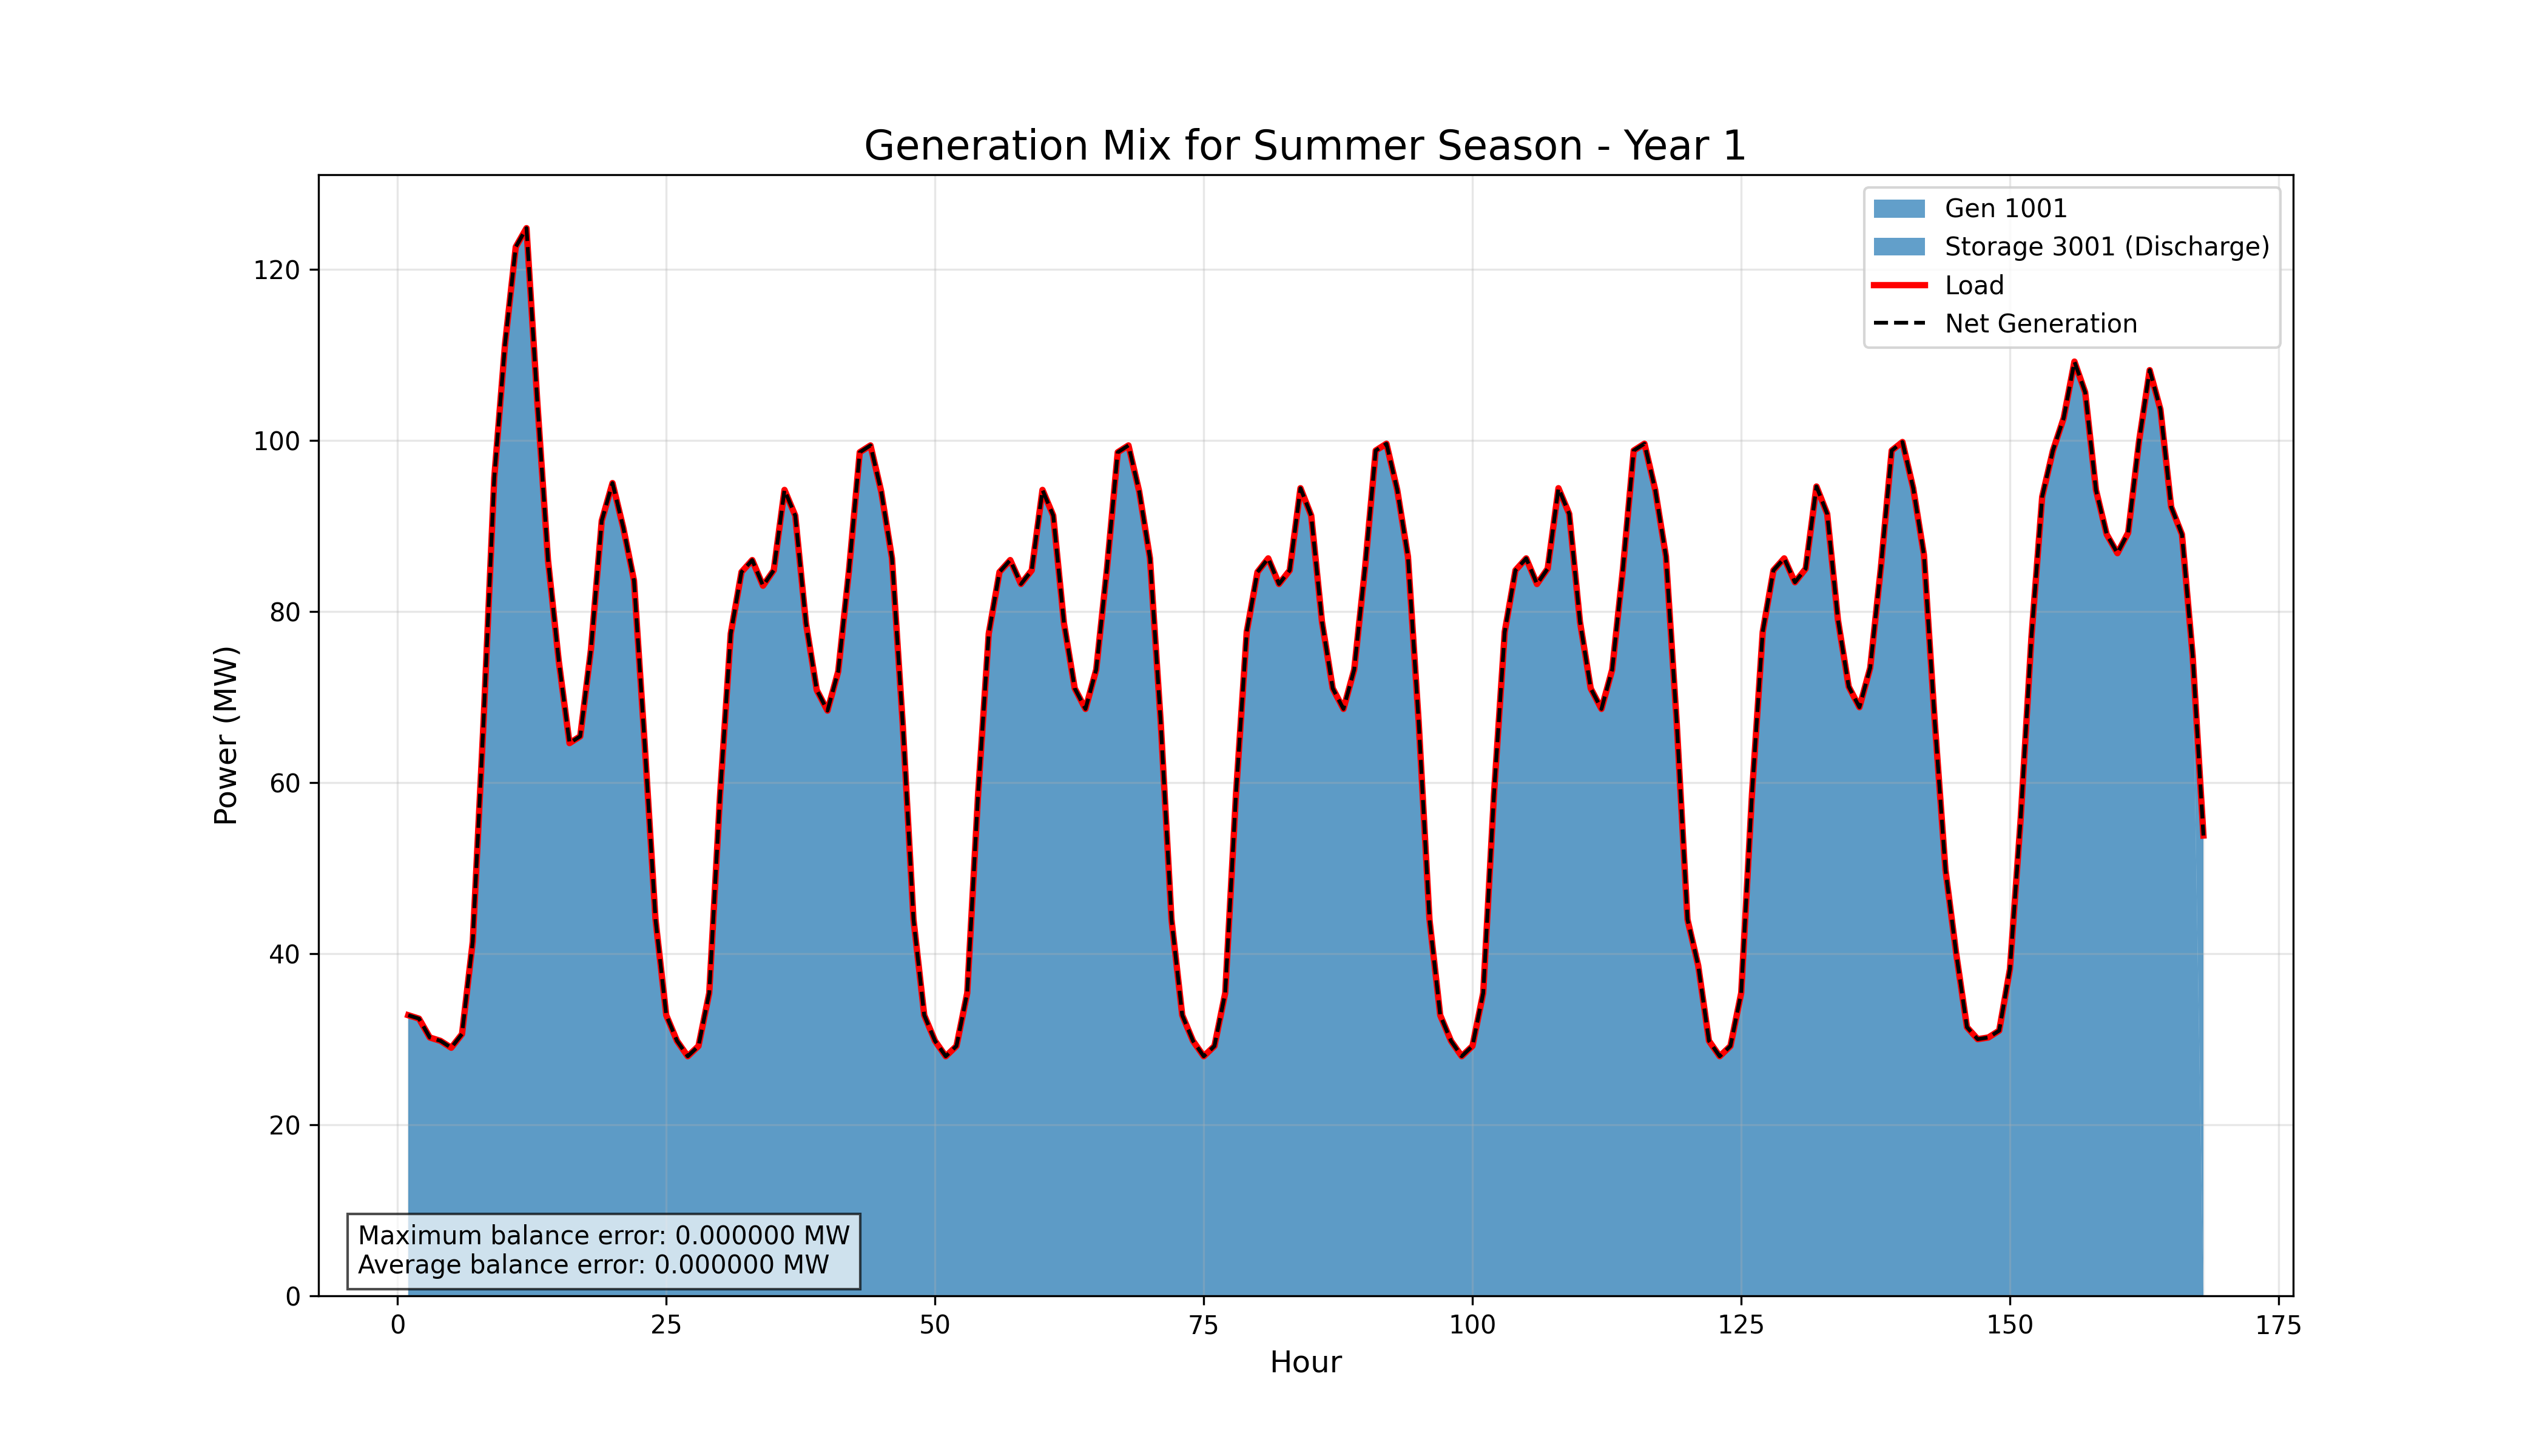
\includegraphics[width=0.85\textwidth]{images/summer_mix_year1.png}
    \caption{Summer week, Year 1}
    \label{fig:summer_mix_year1}
\end{figure}
% Renewables (solar especially) and storage contribute more to 
% the dispatch mix. Thermal units provide baseload and cover cloudy periods or evening peaks
\begin{figure}[h!]
    \centering
    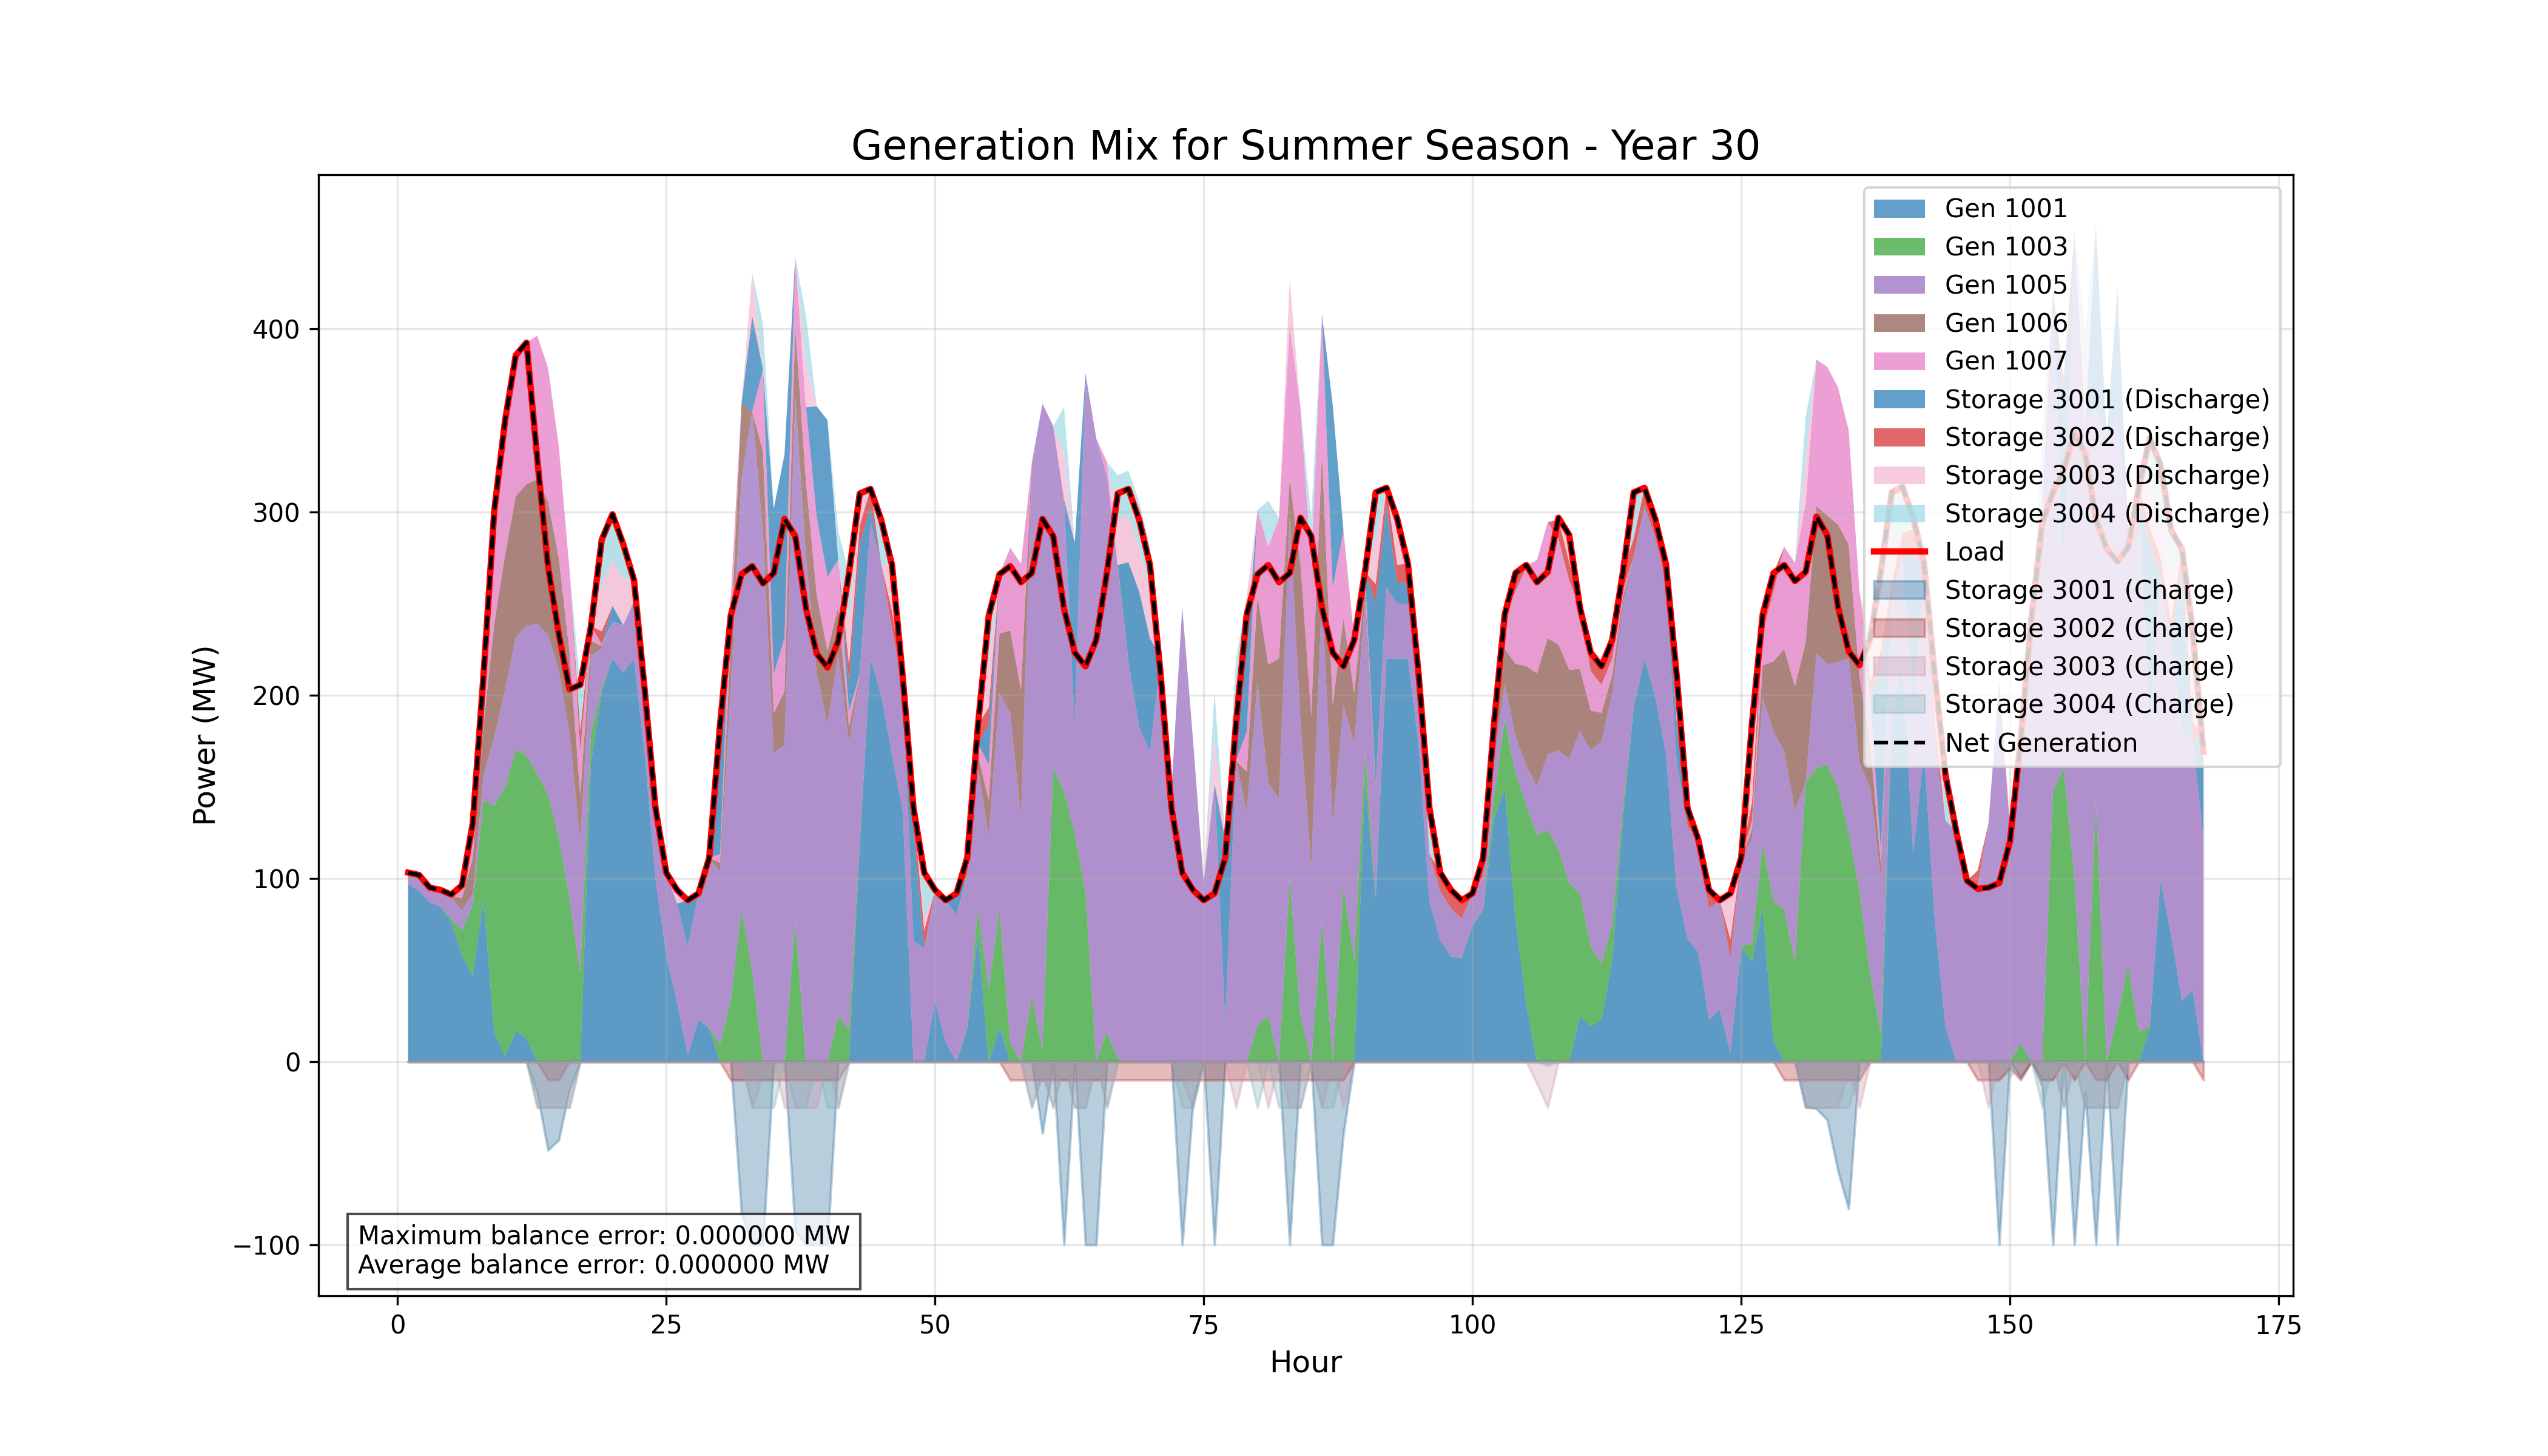
\includegraphics[width=0.85\textwidth]{images/summer_mix_year30.png}
    \caption{Summer week, Year 30}
    \label{fig:summer_mix_year30}
\end{figure}

% A highly diversified dispatch with strong contributions 
% from both solar and storage. Thermal assets run at lower output except during residual 
% peaks or cloudy days.

\textit{Analysis -- Summer Mix}
\vspace{-0.4em}  
\begin{itemize}
    \item Summer dispatch is more balanced, with renewables and storage taking a 
    leading role, especially in Year 30. Solar output is visibly larger, and storage both absorbs 
    surplus and releases it during evening peaks.
    \item Storage shows deep charge/discharge cycles, reflecting its use in 
    smoothing the “duck curve” effect common in high-renewable summer systems.
    \item Thermal assets still cover persistent deficits, but their 
    share is reduced, especially in Year 30, indicating progress toward decarbonization.
    \item If storage is persistently full/empty or solar/wind are curtailed, 
    this could signal network or asset selection limits. Should be investigated. 
    We notice however the storage no longer produce so much surplus as in the first years.
\end{itemize}

\newpage
\textit{Analysis -- Summer vs Winter}
\vspace{-0.4em}
\begin{itemize}
    \item As seen in the 1st version of the model, summer clearly drives renewable assets
    penetration. High solar availability, plays a crucial role there. The detailed dispatch over the years 
    shows that their utilization is economically meaningful with an increase in the load.
    \item The model is able to handle the load growth and the asset aging. It is able to 
    replace the assets at the end of their technical lifetimes and increase the number of assets.
    \item Storage plays a critical, season-dependent role—absorbing midday surplus in summer. 
    As demand grows, even winter periods begin to see sufficient surplus to enable storage cycles, 
    highlighting how higher loads can unlock storage value year-round.
    \item We notice that assets are used to their full potential in winter by the last 
    years of the planning horizon. This highlights not only the solver’s ability to 
    maximize the utilization of existing assets before commissioning new ones, but also 
    demonstrates, on a smaller scale, how even a 3–5\% annual increase in load inevitably 
    drives the need for additional assets and infrastructure.
\end{itemize}

\subsubsection*{D. Discussion}
The MILP framework offers clear advantages over static or LP-based approaches for multi-year grid 
planning, enabling joint optimization of investment and operations while explicitly handling 
asset aging and demand growth. However, several model and code limitations should be noted when 
interpreting the results.


\textit{Limitations}
\vspace{-0.4em}
\begin{itemize}
    \item The use of representative ‘weeks’ for each year speeds up simulation but may miss rare, extreme events 
    (prolonged renewable droughts, spikes in demand, etc.). 
    \item Asset investments are modeled as annual, binary decisions—this simplifies 
    computation but prevents gradual or partial upgrades. 
    \item The model is deterministic, lacking explicit treatment of uncertainty or scenario variation, 
    and does not capture all operational details (e.g., ramping, start-up costs, maintenance downtimes). 
    \item While tractable for this test grid, scalability to larger systems or finer time resolution 
    could be computationally challenging. 
\end{itemize}


\textit{Advantages and Disadvantages}
\vspace{-0.4em}
\begin{itemize}
    \item The main strength is the direct linkage between investment decisions and operational outcomes, 
    allowing transparent tracking of asset utilization and portfolio evolution. 
    \item The candidate-pool method reflects real planning flexibility, and the modular structure 
    supports future extensions. 
    \item The simplified operational and uncertainty modeling, as well as week-based aggregation, 
    may limit realism—especially for system resilience to rare stress events or volatility in demand/generation.
\end{itemize}

\textit{Deeper Analysis and Framework Capabilities}
\vspace{-0.4em}
\begin{itemize}
    \item This framework is well-suited to address core planning questions, such as the marginal 
    value and utilization of storage or renewables, tradeoffs between asset types, and how investments 
    shift as technical/economic limits are reached. 
    \item It can analyze resilience (e.g., under severe winter or renewable drought), track changes 
    in system cost, CO$_2$ emissions, and identify when transmission or asset constraints become critical. 
    \item While perfect foresight is assumed, the model could be extended with scenario or stochastic 
    analysis to improve robustness. 
    \item Further work should also include demand response, multi-objective optimization, and market 
    mechanisms.
\end{itemize}

\textit{Summary}\\
In summary, this MILP approach provides a flexible and technically rigorous tool for long-term planning, 
though simplifications for tractability (week-based aggregation, perfect foresight, annual binary investment) 
and the lack of uncertainty modeling remain key limitations. Despite these, the framework forms a solid basis 
for scenario analysis and deeper strategic investigation as outlined above.

%------------------------------------------
\subsection{Forecasting module}
A series of models were developed and compared for operational forecasting of electricity generation. 
Performance was evaluated over a 7-day period starting 2024-01-01. The principal metrics considered are RMSE, 
MAE, and $R^2$, computed both overall and per day. Table~\ref{tab:forecast-metrics} summarizes the test results 
for all model variants.

\begin{table}[h!]
    \centering
    \begin{tabular}{lccc}
        \textbf{Model} & \textbf{RMSE} & \textbf{MAE} & $\mathbf{R^2}$ \\
        \hline
        A. Time only & 0.130 & 0.070 & 0.095 \\
        B. Time + cyclic features & 0.022 & 0.011 & 0.973 \\
        C. Optimized hyperparameters & 0.022 & 0.013 & 0.973 \\
        D. Recursive \textit{(not used)} & 0.119 & 0.053 & -0.281 \\
        E. 'Optimized set'+ weather features & 0.024 & 0.010 & 0.970 \\
        F. + POA clear-sky & 0.004 & 0.002 & 0.998 \\
    \end{tabular}
    \caption{Forecasting model performance on test set (7 days).}
    \label{tab:forecast-metrics}
\end{table}

%------------------------------------------
\subsubsection*{A. Time Features Only}
The baseline model (A), relying solely on time features, achieved poor predictive performance ($R^2=0.095$), 
with substantial errors for certain days (see daily breakdowns). 

We began with a minimal model using only time-related features (hour and day). This 
provided a simple benchmark and captured regular daily and weekly patterns but did not 
account for weather effects or recent historical trends. It achieved poor performance. 

\begin{figure}[H]
    \centering
    \includegraphics[width=\linewidth]{images/set_time.png}
    \caption{Set 1 - Time features only}
    \label{fig:set1-forecast-profile}
\end{figure}

\begin{table}[H]
    \centering
    \begin{tabular}{lccc}
        Date        & MAE    & RMSE   & R\textsuperscript{2} \\
        \hline
        2024-01-01  & 0.045  & 0.076  & 0.693 \\
        2024-01-02  & 0.098  & 0.169  & -15.138 \\
        2024-01-03  & 0.036  & 0.064  & 0.922 \\
    \end{tabular}
    \caption{Set A - Daily Performance Metrics}
\end{table}

%------------------------------------------
\subsubsection*{B. Time + Lagged Features}
Recognizing the autocorrelated nature of PV output, we next included lagged values of 
electricity generation (e.g., previous hour, previous day, previous week). Incorporating 
these lags enabled the model to better understand night/time patterns (no sub-zero values).
However, significant errors remained on some days, indicating the model's limited ability 
to capture complex temporal dependencies.

\begin{figure}[H]
    \centering
    \includegraphics[width=\linewidth]{images/set_lags.png}
    \caption{Set B - Time + time/cyclical features (before feature selection)}
\end{figure}

\begin{table}[H]
    \centering
    \begin{tabular}{lccc}
        Date        & MAE    & RMSE   & R\textsuperscript{2} \\
        \hline
        2024-01-01  & 0.043  & 0.078  & 0.677 \\
        2024-01-02  & 0.087  & 0.156  & -12.658 \\
        2024-01-03  & 0.037  & 0.069  & 0.908 \\
    \end{tabular}
    \caption{Set 2 - Daily Performance Metrics}
\end{table}

\textbf{Feature Importance Analysis} Understanding which features 
most significantly impact the model's predictions is crucial for 
interpretability and further model refinement. We conducted a feature 
importance analysis by keeping only the most important features in the 
training set.

We conducted  the feature optimization number by using the Bayesian optimization search.
It learns from previous trials, improving efficiency over brute-force methods sucha grid 
search or back-/front- ward elimination which are more expensive.

\begin{figure}[h!]
    \centering
    \includegraphics[width=0.75\linewidth]{images/feature-importance-cyclic.png}
    \caption{Feature Importance derived from the Bayesian optimization search}
    \label{fig:feature-importance}
\end{figure}

The decrease of the error in this step is highly significant. Not only does it 
show that over 95\% of the model's predictive power was explained by just three 
features: \texttt{electricity\_lag1}, \texttt{electricity\_lag24}, and \texttt{hour\_sin} 
but it also highlights the relevance of removing noise (excessive features) in the prediction
to avoid overfitting. 

\begin{figure}[H]
    \centering
    \includegraphics[width=\linewidth]{images/set_lags2.png}
    \caption{Set B - Time + time/cyclical features (after feature selection)}
    \label{fig:set2-forecast-profile}
\end{figure}

\begin{table}[H]
    \centering
    \begin{tabular}{lccc}
        Date        & MAE    & RMSE   & R\textsuperscript{2} \\
        \hline
        2024-01-01  & 0.013  & 0.025  & 0.967 \\
        2024-01-02  & 0.013  & 0.023  & 0.693 \\
        2024-01-03  & 0.012  & 0.019  & 0.993 \\
    \end{tabular}
    \caption{Set 2 - Daily Performance Metrics}
\end{table}

%------------------------------------------
\subsubsection*{C. Parameter tuning and cross-validation}
To evaluate how well your model is likely to perform on unseen data, we performed 
cross validation (evaluation mechanism). It splits the data into several parts (folds), 
trains on some, and tests on others. It should prevent overfitting. It requires a peticular
attention when it comes to time series data so the splits are not randomly picked but rather 
sequential in time.

Hyperparameter tuning is the search process to find the best hyperparameters for the model.
Its robustness is improved. Again, we used a Bayesian optimization search to find the 
best hyperparameters.

\begin{figure}[H]
    \centering
    \includegraphics[width=\linewidth]{images/set_bayesian1.png}
    \caption{Set C - Features selected by Bayesian optimization}
    \label{fig:set3-forecast-profile}
\end{figure}

\begin{table}[H]
    \centering
    \caption{Set 3 - Daily Performance Metrics}
    \begin{tabular}{lccc}
        Date        & MAE    & RMSE   & R\textsuperscript{2} \\
        \hline
        2024-01-01  & 0.009  & 0.023  & 0.972 \\
        2024-01-02  & 0.010  & 0.022  & 0.732 \\
        2024-01-03  & 0.011  & 0.019  & 0.993 \\
    \end{tabular}
\end{table}

Ironically, these steps could lead to overfitting and poor generalization. 
Simultaneous optimization of hyperparameters with limited evaluation 
calls may not fully explore the searchspace, leading to suboptimal solutions. 
These methods are computationally expensive and using too wide ranges or too 
little cv folds may lead to poor results. It's a trade-off between exploration and 
exploitation. 

We see here, that despite the (expensive) cross-validation and hyperparameter tuning, 
the model does not generalize much better than the one with feature selection only. 

%------------------------------------------
\subsubsection*{D. Recursive Prediction}
In operational settings, true future lag values are unknown; predictions must be generated recursively, 
using model outputs as future lag inputs. This recursive prediction (Model D) more accurately reflects 
real-world constraints, but error accumulation can occur, leading to degraded performance.

\begin{figure}[H]
    \centering
    \includegraphics[width=\linewidth]{images/set_recursive.png}
    \caption{Set 4 - Recursive prediction}
    \label{fig:set4-forecast-profile}
\end{figure}

\begin{table}[H]
    \centering
    \begin{tabular}{lccc}
        Date        & MAE    & RMSE   & R\textsuperscript{2} \\
        \hline
        2024-01-01  & 0.080  & 0.160  & -0.353 \\
        2024-01-02  & 0.027  & 0.052  & -0.499 \\
        2024-01-03  & \textit{NaN}    & \textit{NaN}    & \textit{NaN} \\
    \end{tabular}
    \caption{Set 4 - Daily Performance Metrics}
\end{table}

The model seemed successfully implemented including the preprocessing of time-series 
data (removing nighttime hours), aligning input-output sequences, and setting up the loop 
logic to feed previous predictions into future steps. However, the model did not yield 
stable or reliable results. 

It remained flat. This behavior is most likely due error accumulation and feedback saturation, 
where early incorrect low predictions suppress the entire sequence. Broken temporal continuity 
from removing nighttime data, represents a clear challenge in the modeling too. We tried to 
implement the method but not extensive research was done.  

%------------------------------------------
\subsubsection*{E. Enhanced Features with POA Clear-Sky}
Finally, we extended the feature set to include physics-based drivers—specifically, 
plane-of-array (POA) clear-sky irradiance. By combining these weather-driven variables 
with the selected lags and time features, the model could account for both physical 
potential and recent variability, resulting in the best overall performance.

\begin{figure}[H]
    \centering
    \includegraphics[width=\linewidth]{images/set_poa.png}
    \caption{Set 5 - Enhanced features with POA clear-sky}
    \label{fig:set5-forecast-profile}
\end{figure}

\begin{table}[H]
    \centering
    \begin{tabular}{lccc}
        Date        & MAE    & RMSE   & R\textsuperscript{2} \\
        \hline
        2024-01-01  & 0.008  & 0.026  & 0.970 \\
        2024-01-02  & 0.009  & 0.022  & 0.725 \\
        2024-01-03  & 0.015  & 0.028  & 0.985 \\
    \end{tabular}
    \caption{Set 5 - Daily Performance Metrics}
\end{table}

Error and accuracy metrics are improved. However, the model is still far from being perfect 
and computational expense is high for a sole 0.1\% improvement of the MAE-error for the day ahead 
prediction horizon. 

\begin{figure}[H]
    \centering
    \includegraphics[width=0.75\linewidth]{images/feature-importance-weather.png}
    \caption{Feature Importance including weather-features}
    \label{fig:feature-importance-weather}
\end{figure}

We performed a feature selection with the new weather-features based to understand their importance 
compare to the previous time-only-lags. We notice 7 additional "POA"-features in the top 20 and we see 
that within out parameter array seach we manage to quantify the the sum of their importance which 
improves the prediction performance by 0.2\% of the MAE-error. In average POA-features impact is +0.003.

% \subsubsection*{F. }

% \begin{figure}[H]
%     \centering
%     \includegraphics[width=\linewidth]{images/set_xgboost.png}
%     \caption{Set F - XGBoost}
%     \label{fig:set6-forecast-profile}
% \end{figure}

% \begin{table}[H]
%     \centering
%     \begin{tabular}{lccc}
%         Date        & MAE    & RMSE   & R\textsuperscript{2} \\
%         \hline
%         2024-01-01  & 0.002  & 0.004  & 0.999 \\
%         2024-01-02  & 0.001  & 0.003  & 0.996 \\
%         2024-01-03  & 0.003  & 0.006  & 0.999 \\
%     \end{tabular}
%     \caption{Set F - Daily Performance Metrics (XGBoost + Blending)}
% \end{table}


